\documentclass[12pt, a4paper]{report}
\usepackage[utf8]{inputenc}
\usepackage{mathptmx} % Times New Roman
\usepackage{geometry}
\geometry{a4paper, margin=1in}
\usepackage{setspace}
\setstretch{1.5}
\usepackage{graphicx}
\usepackage{titlesec}
\PassOptionsToPackage{hyphens}{url}
\usepackage{hyperref}
\usepackage{fancyhdr}
\usepackage{listings}
\usepackage{xcolor}
\usepackage{tabularx}
\usepackage{booktabs}
\usepackage{longtable}
\usepackage{float}
\usepackage{eso-pic}
\usepackage{tikz}
\usepackage{enumitem}
\usetikzlibrary{calc, shapes.geometric, shapes.multipart, arrows.meta, positioning, fit, backgrounds, decorations.pathreplacing}

% --- PAGE BORDER ---
\definecolor{bordercolor}{HTML}{B3A382} % Khaki/Gold border color matching the Word template
\AddToShipoutPictureBG{%
\begin{tikzpicture}[overlay,remember picture]
\draw[line width=0.5pt, double, double distance=1.5pt, color=bordercolor]
    ($ (current page.north west) + (0.5in,-0.5in) $)
    rectangle
    ($ (current page.south east) + (-0.5in,0.5in) $);
\end{tikzpicture}
}

% --- HEADER & FOOTER ---
\pagestyle{fancy}
\fancyhf{} % Clear defaults
\renewcommand{\headrulewidth}{0pt} % Remove header line
% Set footer for standard pages
\cfoot{\textcolor{blue!60}{\fontsize{9pt}{11pt}\selectfont MIT School of Computing, MIT ADT University}}
\rfoot{\thepage}

% Ensure title pages, certificates, and chapter starting pages also have the footer
\fancypagestyle{empty}{
  \fancyhf{}
  \renewcommand{\headrulewidth}{0pt}
  \cfoot{\textcolor{blue!60}{\fontsize{9pt}{11pt}\selectfont MIT School of Computing, MIT ADT University}}
}
\fancypagestyle{plain}{
  \fancyhf{}
  \renewcommand{\headrulewidth}{0pt}
  \cfoot{\textcolor{blue!60}{\fontsize{9pt}{11pt}\selectfont MIT School of Computing, MIT ADT University}}
  \rfoot{\thepage}
}

% Chapter formatting
\titleformat{\chapter}[display]
  {\normalfont\fontsize{16pt}{19pt}\bfseries\centering}{\chaptertitlename\ \thechapter}{10pt}{\fontsize{16pt}{19pt}\selectfont}
\titlespacing*{\chapter}{0pt}{-20pt}{20pt}
\titleformat{\section}
  {\normalfont\fontsize{14pt}{17pt}\bfseries}{\thesection}{1em}{}
\titleformat{\subsection}
  {\normalfont\fontsize{12pt}{15pt}\bfseries}{\thesubsection}{1em}{}

% Code block styling
\definecolor{codegreen}{rgb}{0,0.6,0}
\definecolor{codegray}{rgb}{0.5,0.5,0.5}
\definecolor{codepurple}{rgb}{0.58,0,0.82}
\definecolor{backcolour}{rgb}{0.95,0.95,0.92}
\definecolor{mitpurple}{HTML}{7030A0} % Deep purple matching Word

\lstdefinestyle{mystyle}{
    backgroundcolor=\color{backcolour},   
    commentstyle=\color{codegreen},
    keywordstyle=\color{blue},
    numberstyle=\tiny\color{codegray},
    stringstyle=\color{codepurple},
    basicstyle=\ttfamily\small,
    breakatwhitespace=false,         
    breaklines=true,                 
    captionpos=b,                    
    keepspaces=true,                 
    numbers=left,                    
    numbersep=5pt,                  
    showspaces=false,                
    showstringspaces=false,
    showtabs=false,                  
    tabsize=2
}
\lstset{style=mystyle}

% Colors for TikZ
\definecolor{primary}{RGB}{225,29,72}
\definecolor{secondary}{RGB}{13,148,136}
\definecolor{accent}{RGB}{245,158,11}
\definecolor{dark}{RGB}{15,23,42}
\definecolor{lightgray}{RGB}{241,245,249}
\definecolor{midgray}{RGB}{148,163,184}
\definecolor{success}{RGB}{16,185,129}
\definecolor{danger}{RGB}{239,68,68}
\definecolor{tablebg}{HTML}{f8fafc}
\definecolor{tableborder}{HTML}{cbd5e1}

\begin{document}
\pagenumbering{roman}

% --- TITLE PAGE ---
\begin{titlepage}
    \centering
    \vspace*{0.5cm}
    
    {\Large \textbf{A JURY PROJECT REPORT}}\\[0.3cm]
    \textit{Submitted in partial fulfillment of the requirements} \\
    \textit{for the award of the degree of}\\[0.3cm]
    
    {\Large \textbf{BACHELOR OF TECHNOLOGY}} \\
    \textit{in} \\
    {\large \textbf{COMPUTER SCIENCE \& ENGINEERING}}\\[0.3cm]
    
    \textcolor{mitpurple}{\textbf{SUBJECT: DATA WAREHOUSING AND DATA MINING (DWDM)}}\\[0.8cm]
    
    {\LARGE \textbf{``Customer Behavioral Analysis and Loan Default Classification''}}\\[0.4cm]
    {\large \textit{A Banking Analytics Data Warehouse on Snowflake with a Streamlit Review Dashboard}}\\[0.8cm]
    
    
\includegraphics[width=0.2\textwidth]{logo.png} \\[0.3cm]
    
    \textbf{SUBMITTED BY:}\\
    Dhanush Pillay \hspace{1cm} ADT24SOCB0765 \\
    Shubhangini Dixit \hspace{0.65cm} ADT24SOCB1156 \\
    Semester: $5^{th}$ Semester / TY BDCE \\[0.5cm]
    
    \textbf{INTERNAL FACULTY GUIDE:}\\
    Dr. Reena Pagare \\
    Department of Computer Science \& Engineering \\[0.5cm]
    
    \vfill
    
    \textbf{DEPARTMENT OF COMPUTER SCIENCE \& ENGINEERING}\\
    \textcolor{mitpurple}{\textbf{MIT ART, DESIGN AND TECHNOLOGY UNIVERSITY, PUNE}}\\
    Loni Kalbhor, Pune, MH, India -- 412201
\end{titlepage}

\newpage
\begin{spacing}{1.35}
\tableofcontents
\end{spacing}
\listoffigures
\listoftables

\clearpage
\phantomsection
\addcontentsline{toc}{chapter}{Abstract}
\begin{center}
    {\huge \textbf{Abstract}}\\[1cm]
\end{center}

The project predicts whether a loan will default using only information that was available before the loan was granted. The data comes from the PKDD'99 Czech banking dataset: 682 loans, 76 defaults (an 11.14\% base rate), and 1,056,320 transactions recorded between 1993 and 1998. The central rule of the project is a strict leakage boundary: no transaction, balance, or account event dated on or after the loan date is used to build a predictive feature.

The work covers the full path from raw CSV extracts to a Snowflake data warehouse, a leakage-safe feature mart, six classifiers compared under repeated cross-validation, association-rule mining, behavioural segmentation, and an eight-page Streamlit review dashboard. The warehouse follows a Kimball galaxy schema with two fact tables sharing five conformed dimensions, deployed in Snowflake as a RAW staging layer and a MART layer of modelled tables and reporting views.

The selected classifier is a tuned Gradient Boosting model with repeated cross-validation F1 of $0.571 \pm 0.120$, average precision $0.654$, and ROC AUC $0.864$. Random Forest is statistically tied on F1 and leads on average precision and ROC AUC, so the result is best read as a leading pair rather than a single dominant algorithm. The strongest signal is the customer's balance before the loan; age and gender carry almost no predictive value. A simple balance screen below CZK 20,000 flags 97 of 682 applications and catches 34 of the 76 defaults, at 35.1\% precision against the 11.1\% base rate. The intended use of the model is a review queue, not an automatic rejection rule.

\clearpage
\pagenumbering{arabic}

\chapter{Introduction}
\section{Problem Definition}
Banks hold detailed records of every account transaction, but turning those records into a decision about a loan application is a different problem. A bank wants to prioritise manual review of applications that are likely to default, so that reviewers spend their time where it matters. The target is binary: a loan labelled \texttt{0} was completed or is running without payment problems, while a loan labelled \texttt{1} was completed unpaid or is running in debt.

The modelling rule is stricter than the prediction task itself. No transaction, balance, or account event dated on or after the loan date may be used to build a predictive feature. A model that violates this rule would score well in development and fail in practice, because it would be reading information that did not exist at decision time. This leakage constraint shapes the warehouse design, the feature mart, and every evaluation reported in this document.

\section{Project Objectives}
The objective is an end-to-end analytics system over the PKDD'99 Czech banking dataset: 682 loans, 76 of them defaults (11.14\%), and 1,056,320 transactions from 1993 to 1998. Specifically, the project aims to:

\begin{enumerate}
    \item Design a Kimball-style galaxy schema that stores loan and transaction facts against conformed date, branch, customer, account, and loan-type dimensions.
    \item Deploy the warehouse in Snowflake with a RAW staging layer and a MART layer of modelled tables and reporting views.
    \item Build a leakage-safe feature mart in which every behavioural feature uses only transactions strictly before the loan date.
    \item Compare six supervised classifiers under repeated cross-validation and select a review model with an explicit metric rule.
    \item Mine association rules and behavioural segments that can be read alongside the model score.
    \item Deliver the results through a Streamlit dashboard that supports review, not just reporting.
\end{enumerate}

\section{Scope and Data Boundary}
The source is a historical, anonymised dataset. It contains no loan product category and no interest rate, so the warehouse keeps a single explicit ``Unspecified'' loan-type member and a null rate rather than inventing values. Branch labels are derived from Czech district names. The dataset is small by modern credit-risk standards, and this project treats the result as a historical demonstration of a method, not as a deployable credit policy.

\section{Report Organization}
Chapter~2 reviews the dataset and the relevant background. Chapter~3 describes the system architecture, Chapter~4 the Snowflake deployment, and Chapter~5 the warehouse design. Chapter~6 covers the supervised learning dataset and leakage control, Chapter~7 pattern mining, Chapter~8 classification, and Chapter~9 clustering. Chapter~10 presents the dashboard, and Chapter~11 concludes. Appendix~A maps each end-semester jury rubric item to its section and dashboard page.

\chapter{Literature Review \& Background}
\section{The PKDD '99 Financial Dataset (Berka Dataset)}
This project uses the \textbf{PKDD '99 Financial Dataset}, also known as the \textbf{Berka Dataset}. It contains anonymized real world financial data from a Czech bank. The data was first released for the Discovery Challenge at the 1999 European Conference on Principles of Data Mining and Knowledge Discovery.

\subsection*{Background and Purpose}
The bank originally collected this data to improve customer service and manage risk. They wanted to understand customer behavior better, specifically to identify "good" clients for new financial products and "bad" clients who might default on their loans.

\subsection*{Relational Structure}
The raw data is highly normalized and spread across several interconnected files:
\begin{itemize}
    \item \textbf{Clients (\texttt{client.csv}):} Demographic details of the bank's customers.
    \item \textbf{Accounts (\texttt{account.csv}):} Static details about the accounts, like when they were created.
    \item \textbf{Dispositions (\texttt{disp.csv}):} A mapping table that connects clients to accounts and shows their permissions, like OWNER or DISPONENT.
    \item \textbf{Transactions (\texttt{trans.csv}):} A large table with historical records of all account transactions, including deposits and withdrawals.
    \item \textbf{Loans (\texttt{loan.csv}):} Details on granted loans, including the amount, duration, and final status.
    \item \textbf{Demographics (\texttt{district.csv}):} Socioeconomic statistics for the districts where the clients live.
\end{itemize}

\subsection*{Use in Analytics}
The PKDD '99 dataset is a common benchmark in data science because it has a complex structure and long transaction histories. Researchers often use it for \textbf{relational data mining} and predictive modeling, such as forecasting loan defaults based on past transactions. In this project, we transform this normalized data into a dimensional model so that loan and transaction histories can be queried against the same dates, accounts, and branches.

\section{Dimensional Modeling}
Dimensional modeling is a design technique for data warehouses introduced by Ralph Kimball. It structures data into fact tables (measurements) and dimension tables (context), enabling intuitive querying and high performance for BI tools. A \textit{star schema} has one fact table surrounded by dimension tables. When several fact tables share the same conformed dimensions, the design is called a \textit{galaxy schema}. This project uses a galaxy schema so that loan metrics and transaction metrics can be analysed together.

\section{Credit Risk and Default Prediction}
Credit-risk modelling usually separates a good loan from a default using application data and prior account behaviour. Classical approaches include scored card models, decision trees, and ensemble methods such as random forests and gradient boosting. A recurring finding across this family of work is that recent balance and cash-flow behaviour carry more signal than demographics. This project follows that line: balance-derived features lead the model, while age and gender contribute almost nothing and are retained only as a documented baseline input.

\section{Leakage in Predictive Modelling}
A predictive model must not see information that was unavailable at scoring time. In a loan setting this means every behavioural feature has to be computed from transactions strictly earlier than the loan date. Leakage can enter subtly, for example by scaling on the full dataset before splitting, or by aggregating all transactions of an account and attaching the same vector to every loan. This project addresses both forms: the feature mart uses a date-bounded join, and all scaling and resampling live inside the fitted scikit-learn pipeline so that each validation fold is transformed from its own training data only.

\section{Association Rules and Clustering}
Association-rule mining finds implications such as ``negative balance implies default''. Apriori uses a candidate-generation level-wise search, while FP-Growth compresses transactions into a frequent-pattern tree and avoids candidate generation. Both are run here over pre-loan behaviour baskets so that the two algorithms can be compared on the same data. Clustering complements the supervised model by grouping loans without looking at the default label. K-Means, K-Medoids, AGNES, and DBSCAN represent partitional, medoid-based, hierarchical, and density-based approaches respectively, and are compared on the same standardised feature matrix.

\chapter{System Architecture}
\section{Data Warehouse Architecture}
The system follows a Kimball bottom-up design: raw extracts are staged in Snowflake \texttt{RAW}, the conformed dimensions and facts are deployed to Snowflake \texttt{MART}, and the analytics layer and Streamlit dashboard consume them. The stages are:

\begin{enumerate}
    \item \textbf{Source Systems:} The six raw CSV files of the PKDD dataset (clients, accounts, dispositions, transactions, loans, and district demographics).
    \item \textbf{Staging:} The \texttt{RAW} schema in Snowflake holds five untouched extracts with source row counts; the district file is used to derive branch labels.
    \item \textbf{Data Warehouse:} The \texttt{MART} schema holds the five conformed dimensions, the two fact tables, the analytics tables, and the reporting views.
    \item \textbf{Analytics Layer:} A leakage-safe feature mart, trained model scores, association rules, and cluster labels are written back to \texttt{MART}.
    \item \textbf{Presentation:} A Streamlit application reads the modelled tables and saved artifacts to render eight interactive review pages.
\end{enumerate}

\begin{figure}[H]
    \centering
    \resizebox{\textwidth}{!}{
    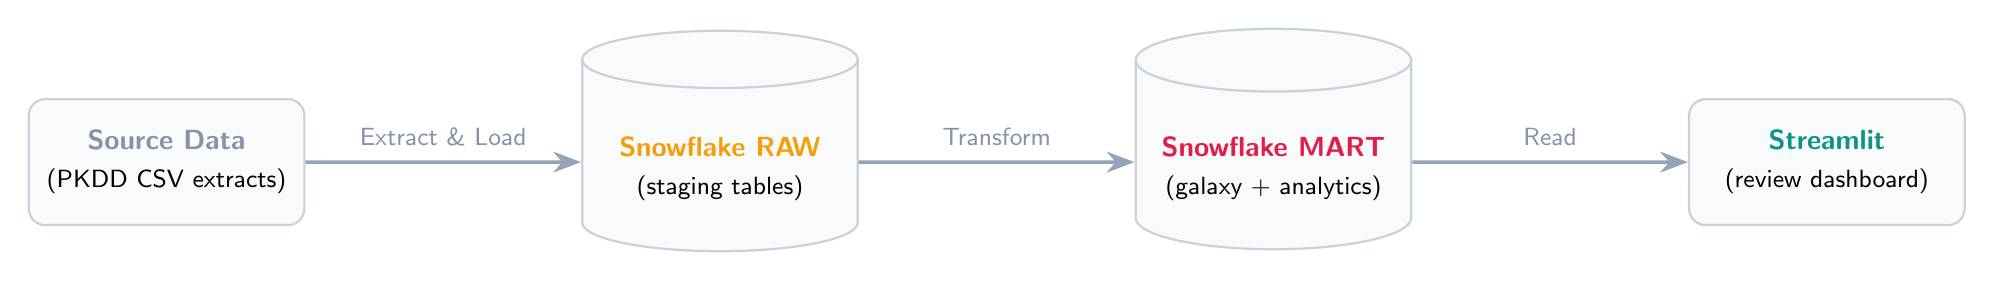
\begin{tikzpicture}[
        node distance=3.5cm,
        every node/.style={font=\sffamily},
        % Standard box
        box/.style={rectangle, draw=midgray!50, thick, fill=white, minimum width=3.5cm, minimum height=1.6cm, align=center, rounded corners=6pt},
        % Database cylinder
        db/.style={cylinder, draw=midgray!50, thick, fill=white, shape border rotate=90, aspect=0.25, minimum width=3.5cm, minimum height=2.8cm, align=center, inner sep=5pt},
        % Arrow style
        arrow/.style={-{Stealth[scale=1.2]}, very thick, color=midgray},
        % Label style
        lbl/.style={above, yshift=2pt, font=\small\sffamily, color=midgray!90!black}
    ]
        
        \node[box, fill=tablebg] (source) {
            \textbf{\textcolor{midgray!90!black}{Source Data}}\\[2pt]
            \small(PKDD CSV extracts)
        };
        
        \node[db, fill=tablebg, right=of source] (raw) {
            \vspace{0.3cm}\\
            \textbf{\textcolor{accent}{Snowflake RAW}}\\[2pt]
            \small(staging tables)
        };
        
        \node[db, fill=tablebg, right=of raw] (mart) {
            \vspace{0.3cm}\\
            \textbf{\textcolor{primary}{Snowflake MART}}\\[2pt]
            \small(galaxy + analytics)
        };
        
        \node[box, fill=tablebg, right=of mart] (bi) {
            \textbf{\textcolor{secondary}{Streamlit}}\\[2pt]
            \small(review dashboard)
        };
        
        \draw[arrow] (source) -- node[lbl] {Extract \& Load} (raw);
        \draw[arrow] (raw) -- node[lbl] {Transform} (mart);
        \draw[arrow] (mart) -- node[lbl] {Read} (bi);
        
    \end{tikzpicture}
    }
    \caption{Bottom-up warehouse architecture on Snowflake with a Streamlit presentation layer}
    \label{fig:architecture}
\end{figure}

The full pipeline is expanded in Figure~\ref{fig:system_arch}. Five source extracts are staged in \texttt{RAW}; the district file is used to label branches. The conformed dimensions and two fact tables are deployed to \texttt{MART}, followed by the leakage-safe analytics tables, and the Streamlit dashboard reads those modelled tables directly. No reporting tool sits between the warehouse and the browser.

\begin{figure}[H]
    \centering
    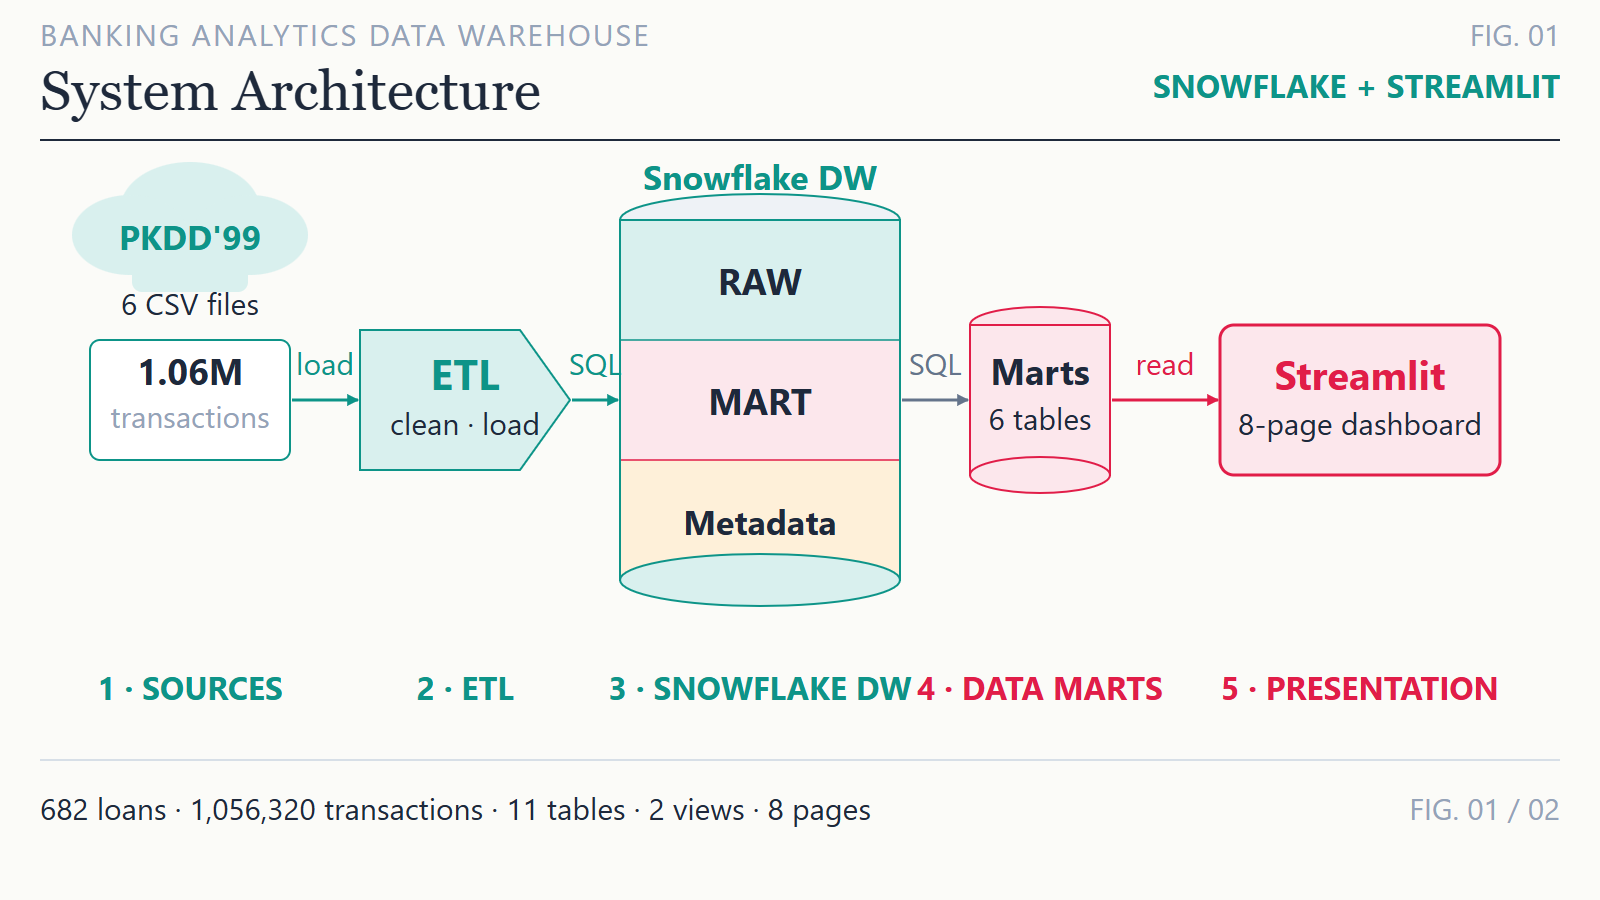
\includegraphics[width=0.95\textwidth]{figures/01_system_architecture.png}
    \caption{End-to-end Snowflake pipeline from raw extracts to the Streamlit review dashboard}
    \label{fig:system_arch}
\end{figure}

\begin{figure}[H]
    \centering
    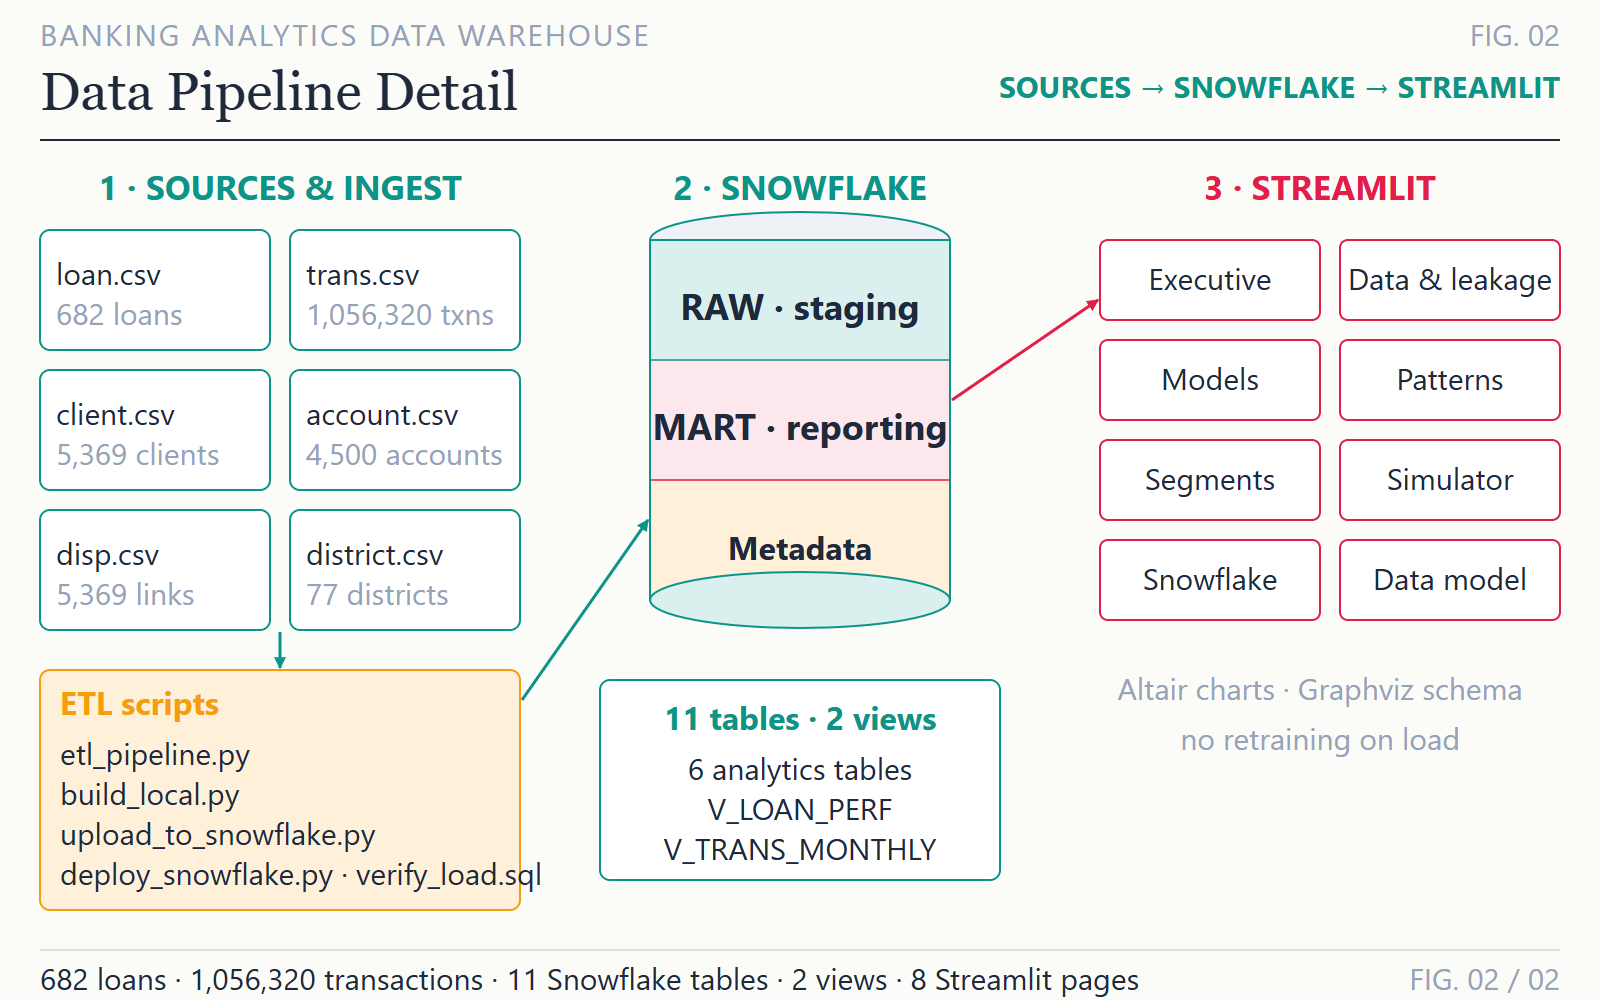
\includegraphics[width=0.95\textwidth]{figures/02_data_pipeline.png}
    \caption{Pipeline detail: the six source extracts, the ETL scripts, the Snowflake RAW and MART layers, and the eight Streamlit pages}
    \label{fig:pipeline_detail}
\end{figure}

\section{Requirement Analysis}
The following requirements drove the design:
\begin{itemize}
    \item \textbf{Data Integration:} Extract the historical banking data, stage it without modification, and load a central modelled repository with repeatable scripts.
    \item \textbf{Dimensional Modelling:} Support slicing across time, geography (district/branch), and customer demographics through conformed dimensions.
    \item \textbf{Metric Calculation:} Produce loan default rates, balance-derived behaviour measures, and segment summaries from the same warehouse.
    \item \textbf{Leakage Control:} Every predictive feature must be computed from pre-loan transactions only, and the condition must be verified automatically.
    \item \textbf{Review Support:} Expose scores, rules, and segment labels through an interactive dashboard rather than a static report.
\end{itemize}

\section{Technology Stack}
The implementation uses Python and pandas for extraction and transformation, Snowflake for the warehouse, scikit-learn for classification and clustering, mlxtend for Apriori and FP-Growth, Altair and Graphviz for dashboard visuals, and Streamlit for the application layer. Loader scripts create or replace objects and truncate target tables before writing, so a rerun does not append duplicate rows.

\section{ETL Validation and Data Integrity}
The transformation stage handles null values, parses date strings into standard date keys, generates surrogate identifiers, and casts financial amounts to numeric types. To prove that no records are lost during extraction and load, row counts are reconciled between the source files and the loaded warehouse tables.

\begin{table}[H]
    \centering
    \begin{tabular}{|l|c|c|c|}
        \hline
        \textbf{Entity} & \textbf{Raw CSV Rows} & \textbf{Loaded DB Rows} & \textbf{Accuracy Match} \\
        \hline
        Transactions & 1,056,320 & 1,056,320 & 100\% \\
        Loans & 682 & 682 & 100\% \\
        Accounts & 4,500 & 4,500 & 100\% \\
        Customers & 5,369 & 5,369 & 100\% \\
        \hline
    \end{tabular}
    \caption{ETL data reconciliation and accuracy proof}
    \label{tab:etl_accuracy}
\end{table}

Referential integrity is enforced by checks that each fact row resolves to a valid dimension key. The build also verifies that the number of feature rows equals the number of loan facts, and that no feature row contains post-loan transaction activity.

\chapter{Snowflake Deployment}
\section{Deployment Overview}
The warehouse is deployed in Snowflake as the database \texttt{LOAN\_DEFAULT\_DW}, served by the virtual warehouse \texttt{PBI\_WH}. Two schemas separate raw staging from modelled data: \texttt{RAW} holds the five source extracts, and \texttt{MART} holds the conformed dimensions, facts, analytics tables, and reporting views. This split keeps the source records auditable while giving the dashboard a stable set of modelled objects.

\begin{table}[H]
    \centering
    \small
    \renewcommand{\arraystretch}{1.15}
    \begin{tabularx}{\textwidth}{|l|l|r|X|}
        \hline
        \textbf{Schema} & \textbf{Object} & \textbf{Expected rows} & \textbf{Purpose} \\
        \hline
        RAW & \texttt{RAW\_LOAN} & 682 & Loan extract \\
        RAW & \texttt{RAW\_TRANS} & 1,056,320 & Transaction extract \\
        RAW & \texttt{RAW\_CLIENT} & 5,369 & Client extract \\
        RAW & \texttt{RAW\_ACCOUNT} & 4,500 & Account extract \\
        RAW & \texttt{RAW\_DISP} & 5,369 & Client--account disposition \\
        MART & \texttt{DIM\_DATE} & 2,191 & Calendar dimension, 1993--1998 \\
        MART & \texttt{DIM\_BRANCH} & 77 & Branch (district) dimension \\
        MART & \texttt{DIM\_CUSTOMER} & 5,369 & Customer dimension \\
        MART & \texttt{DIM\_ACCOUNT} & 4,500 & Account dimension \\
        MART & \texttt{DIM\_LOAN\_TYPE} & 1 & Loan product dimension \\
        MART & \texttt{FACT\_LOANS} & 682 & Loan fact, one row per loan \\
        MART & \texttt{FACT\_TRANSACTIONS} & 1,056,320 & Transaction fact, one row per transaction \\
        MART & \texttt{MART\_LOAN\_FEATURES} & 682 & Leakage-safe feature mart \\
        MART & \texttt{MART\_MODEL\_SCORES} & 682 & Out-of-fold review scores \\
        MART & \texttt{MART\_LOAN\_SEGMENTS} & 682 & K-Means segment labels \\
        MART & \texttt{MART\_LOAN\_RISK} & 682 & Features, score, and segment \\
        MART & \texttt{MART\_CLUSTER\_LABELS} & 682 & Four clustering methods \\
        MART & \texttt{MART\_CLUSTERING\_COMPARISON} & 4 & Clustering metrics and verdict \\
        MART & \texttt{V\_LOAN\_PERF} & view & Loan performance with score and segment \\
        MART & \texttt{V\_TRANS\_MONTHLY} & view & Pre-loan transaction monthly rollup \\
        \hline
    \end{tabularx}
    \caption{Snowflake objects: 18 tables and 2 reporting views}
    \label{tab:snowflake_objects}
\end{table}

\section{Loading and Verification}
The DDL script creates the warehouse, database, schemas, tables, and views. The upload script reads the exported CSV extracts and the seven star-schema tables from the local DuckDB warehouse, truncates each target table before writing, and loads five RAW tables plus thirteen MART tables. Because every target is cleared first, repeated runs are idempotent and cannot double-count rows. A separate verification script compares loaded row counts against the expected values and previews the reporting views.

Row counts matched exactly after deployment: 682 loans, 1,056,320 transactions, 5,369 clients, 4,500 accounts, 2,191 calendar days, 77 branches, one loan-type member, and 682 rows in each per-loan analytics table. These figures agree with the source reconciliation in Table~\ref{tab:etl_accuracy}.

\section{Reporting Views}
Two views give reviewers a ready-made analytic surface:
\begin{itemize}
    \item \texttt{V\_LOAN\_PERF} joins the feature mart, model scores, and segment labels into one row per loan. It adds a risk quadrant from loan amount and balance at loan, and a low-balance flag for balance below CZK 20,000.
    \item \texttt{V\_TRANS\_MONTHLY} aggregates pre-loan transactions to one row per account and month. The \texttt{WHERE} clause keeps only transactions strictly before the loan date, so the view preserves the same leakage boundary as the feature mart.
\end{itemize}

\section{Dashboard Connectivity}
The Streamlit application can read the six modelled MART tables directly from Snowflake while keeping model metrics, pattern outputs, and the data-model card on local artifacts. Access uses a Programmatic Access Token paired with a network policy, so the dashboard does not prompt for a multi-factor code on every refresh. The Snowflake page of the dashboard documents the RAW/MART split, shows expected and live row counts, previews the two views, and displays the verification SQL.

\begin{figure}[H]
    \centering
    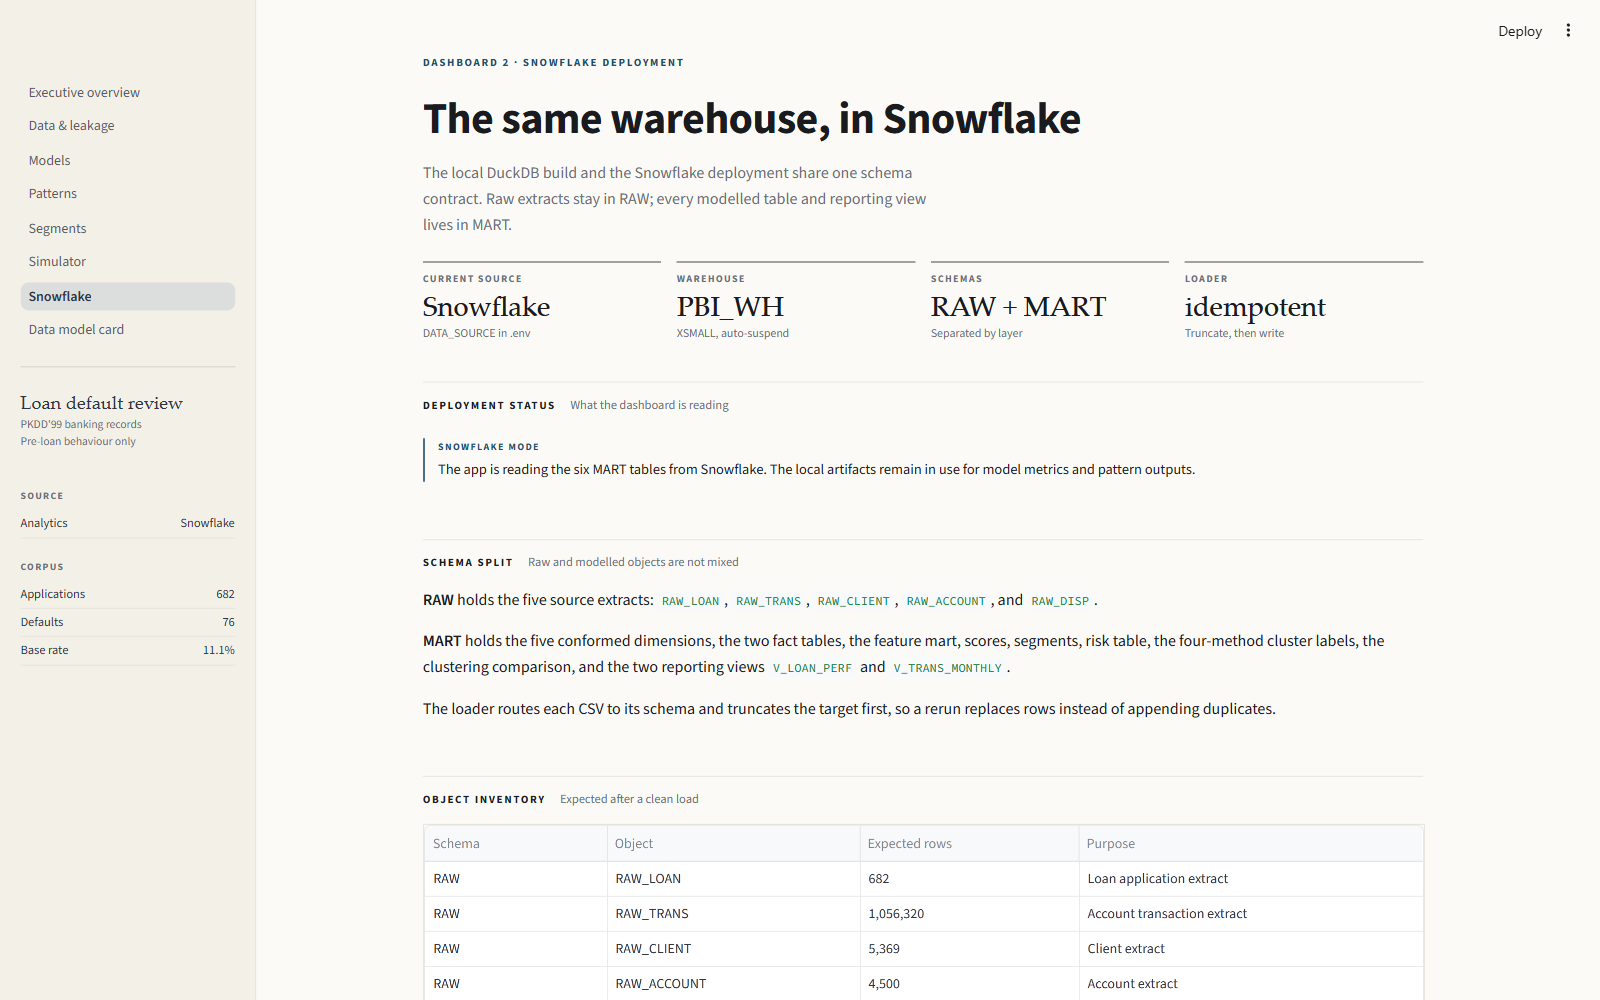
\includegraphics[width=0.92\textwidth]{figures/27_dashboard_snowflake.png}
    \caption{Streamlit dashboard: Snowflake deployment page}
    \label{fig:snowflake_page}
\end{figure}

\chapter{Data Warehouse Design and Implementation}
\section{Source Database Design}
In the raw operational form, answering a question such as ``what is the default rate for a given district and loan-size band?'' requires joining several normalised tables and re-deriving every measure each time. The source CSVs were parsed, mapped to common keys, and cleaned before being loaded into the target warehouse schema. The dimensional model separates measurements (facts) from context (dimensions), so the same measures can be reused across different analyses.

\section{Dimensional Modeling (Galaxy Schema)}
To accommodate both transaction metrics and loan metrics, a \textbf{Galaxy Schema} was implemented: an advanced evolution of the star schema in which multiple fact tables share conformed dimensions. Each fact table with its dimensions forms a star; together the two stars form a galaxy, allowing loan and transaction behaviour to be compared on the same date, account, and branch.

\subsection{Dimension Tables (Context)}
\begin{itemize}
    \item \texttt{dim\_date}: Conformed date dimension covering 2,191 days (year, quarter, month, day, weekday, weekend flag).
    \item \texttt{dim\_branch}: 77 district/branch rows with city, region, and urban/rural type.
    \item \texttt{dim\_customer}: 5,369 clients with age, age group, gender, and home branch.
    \item \texttt{dim\_account}: 4,500 accounts with owner, account type, and open date.
    \item \texttt{dim\_loan\_type}: A single explicit \texttt{Unspecified} member, because the source contains no loan product category or interest rate.
\end{itemize}

\subsection{Fact Tables (Measurements)}
\begin{itemize}
    \item \texttt{fact\_transactions}: 1,056,320 rows, one per account transaction. Grain is the individual transaction; measures are amount and resulting balance.
    \item \texttt{fact\_loans}: 682 rows, one per loan. Measures are principal amount, duration, payments, and status. The interest-rate column is present but null for every row.
\end{itemize}

\begin{table}[H]
    \centering
    \renewcommand{\arraystretch}{1.3}
    \begin{tabularx}{\textwidth}{|>{\raggedright\arraybackslash}l|>{\raggedright\arraybackslash}l|>{\raggedright\arraybackslash}X|}
        \hline
        \textbf{Column Name} & \textbf{Data Type} & \textbf{Description} \\
        \hline
        \texttt{transaction\_id} & \texttt{BIGINT} (PK) & Unique identifier for the transaction. \\
        \texttt{account\_id} & \texttt{INT} (FK) & Reference to \texttt{dim\_account}. \\
        \texttt{date\_id} & \texttt{INT} (FK) & Reference to \texttt{dim\_date} for the transaction date. \\
        \texttt{branch\_id} & \texttt{INT} (FK) & Reference to \texttt{dim\_branch} for the account's district. \\
        \texttt{transaction\_type} & \texttt{VARCHAR} & Deposit or Withdrawal. \\
        \texttt{amount} & \texttt{NUMERIC} & Transaction amount. \\
        \texttt{balance} & \texttt{NUMERIC} & Account balance after the transaction. \\
        \hline
    \end{tabularx}
    \caption{Data dictionary: \texttt{fact\_transactions}}
    \label{tab:dict_transactions}
\end{table}

\begin{table}[H]
    \centering
    \renewcommand{\arraystretch}{1.3}
    \begin{tabularx}{\textwidth}{|>{\raggedright\arraybackslash}l|>{\raggedright\arraybackslash}l|>{\raggedright\arraybackslash}X|}
        \hline
        \textbf{Column Name} & \textbf{Data Type} & \textbf{Description} \\
        \hline
        \texttt{loan\_id} & \texttt{INT} (PK) & Unique identifier for the loan record. \\
        \texttt{account\_id} & \texttt{INT} (FK) & Reference to \texttt{dim\_account}. \\
        \texttt{customer\_id} & \texttt{INT} (FK) & Reference to \texttt{dim\_customer} for the account owner. \\
        \texttt{branch\_id} & \texttt{INT} (FK) & Reference to \texttt{dim\_branch}. \\
        \texttt{loan\_type\_id} & \texttt{INT} (FK) & Reference to \texttt{dim\_loan\_type} (always the Unspecified member). \\
        \texttt{date\_id} & \texttt{INT} (FK) & Reference to \texttt{dim\_date} for the loan date. \\
        \texttt{amount} & \texttt{NUMERIC} & Principal disbursed. \\
        \texttt{tenure\_months} & \texttt{INT} & Agreed loan duration. \\
        \texttt{payments} & \texttt{INT} & Number of instalments. \\
        \texttt{status} & \texttt{VARCHAR} & Closed, Active, or Defaulted. \\
        \hline
    \end{tabularx}
    \caption{Data dictionary: \texttt{fact\_loans}}
    \label{tab:dict_loans}
\end{table}

\begin{figure}[H]
    \centering
    \resizebox{\textwidth}{!}{
    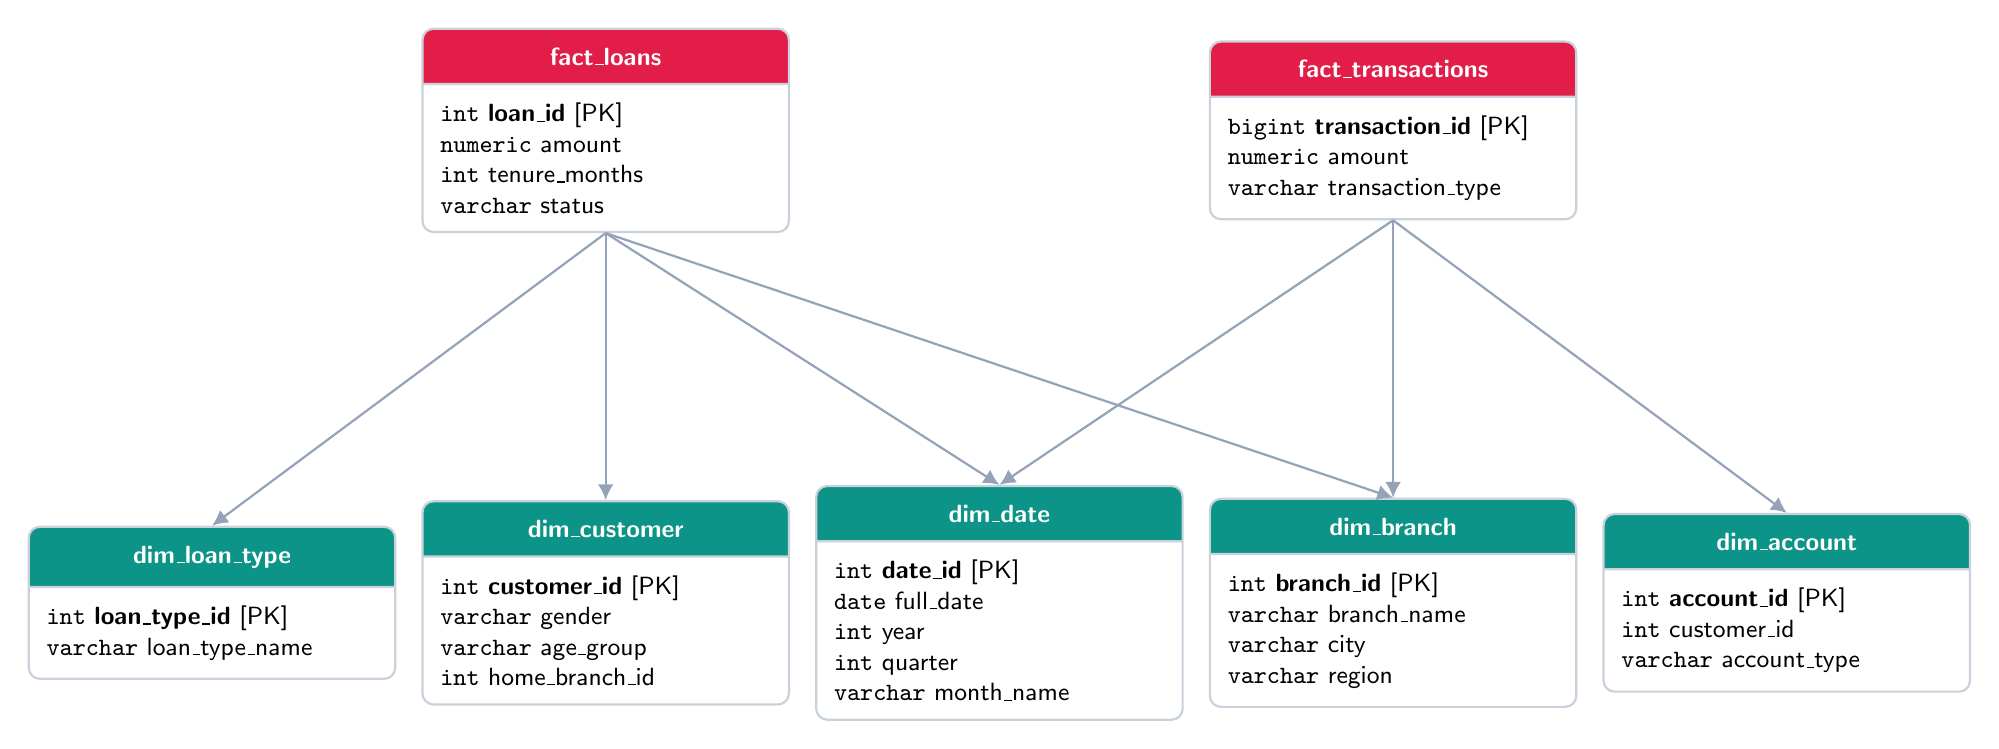
\begin{tikzpicture}[
        >=Stealth,
        every node/.style={font=\sffamily\small},
        tablePrimary/.style={
            rectangle split, rectangle split parts=2,
            draw=midgray!50, thick,
            rectangle split part fill={primary, white},
            rounded corners=4pt, text width=4.2cm, align=left,
            inner sep=1.5ex
        },
        tableSecondary/.style={
            rectangle split, rectangle split parts=2,
            draw=midgray!50, thick,
            rectangle split part fill={secondary, white},
            rounded corners=4pt, text width=4.2cm, align=left,
            inner sep=1.5ex
        },
        line/.style={draw, thick, color=midgray, -{Latex[length=2mm, width=2mm]}}
    ]

    % Fact Loans
    \node[tablePrimary] (floans) at (-4, 6) {
        \hfil \textbf{\textcolor{white}{fact\_loans}} \hfil
        \nodepart{two}
        \texttt{int} \textbf{loan\_id} [PK]\\
        \texttt{numeric} amount\\
        \texttt{int} tenure\_months\\
        \texttt{varchar} status
    };

    % Fact Transactions
    \node[tablePrimary] (ftrans) at (6, 6) {
        \hfil \textbf{\textcolor{white}{fact\_transactions}} \hfil
        \nodepart{two}
        \texttt{bigint} \textbf{transaction\_id} [PK]\\
        \texttt{numeric} amount\\
        \texttt{varchar} transaction\_type
    };

    % Dim Loan Type
    \node[tableSecondary] (dltype) at (-9, 0) {
        \hfil \textbf{\textcolor{white}{dim\_loan\_type}} \hfil
        \nodepart{two}
        \texttt{int} \textbf{loan\_type\_id} [PK]\\
        \texttt{varchar} loan\_type\_name
    };

    % Dim Customer
    \node[tableSecondary] (dcust) at (-4, 0) {
        \hfil \textbf{\textcolor{white}{dim\_customer}} \hfil
        \nodepart{two}
        \texttt{int} \textbf{customer\_id} [PK]\\
        \texttt{varchar} gender\\
        \texttt{varchar} age\_group\\
        \texttt{int} home\_branch\_id
    };

    % Dim Date
    \node[tableSecondary] (ddate) at (1, 0) {
        \hfil \textbf{\textcolor{white}{dim\_date}} \hfil
        \nodepart{two}
        \texttt{int} \textbf{date\_id} [PK]\\
        \texttt{date} full\_date\\
        \texttt{int} year\\
        \texttt{int} quarter\\
        \texttt{varchar} month\_name
    };

    % Dim Branch
    \node[tableSecondary] (dbranch) at (6, 0) {
        \hfil \textbf{\textcolor{white}{dim\_branch}} \hfil
        \nodepart{two}
        \texttt{int} \textbf{branch\_id} [PK]\\
        \texttt{varchar} branch\_name\\
        \texttt{varchar} city\\
        \texttt{varchar} region
    };

    % Dim Account
    \node[tableSecondary] (dacc) at (11, 0) {
        \hfil \textbf{\textcolor{white}{dim\_account}} \hfil
        \nodepart{two}
        \texttt{int} \textbf{account\_id} [PK]\\
        \texttt{int} customer\_id\\
        \texttt{varchar} account\_type
    };

    % Relations (Fact Loans)
    \draw[line] (floans.south) -- (dltype.north);
    \draw[line] (floans.south) -- (dcust.north);
    \draw[line] (floans.south) -- (ddate.north);
    \draw[line] (floans.south) -- (dbranch.north);

    % Relations (Fact Transactions)
    \draw[line] (ftrans.south) -- (ddate.north);
    \draw[line] (ftrans.south) -- (dbranch.north);
    \draw[line] (ftrans.south) -- (dacc.north);

    \end{tikzpicture}
    }
    \caption{Galaxy schema for the banking data warehouse}
    \label{fig:galaxy_schema}
\end{figure}

\section{Warehouse Implementation}
The ETL pipeline builds dimensions first and facts second, so every fact row resolves to a surrogate dimension key. The generated warehouse diagram is shown in Figure~\ref{fig:galaxy_png}; the dashboard data-model card, which lists join keys and a column dictionary for the warehouse tables, is shown in Chapter~10 as Figure~\ref{fig:dashboard_datacard}.

\begin{figure}[H]
    \centering
    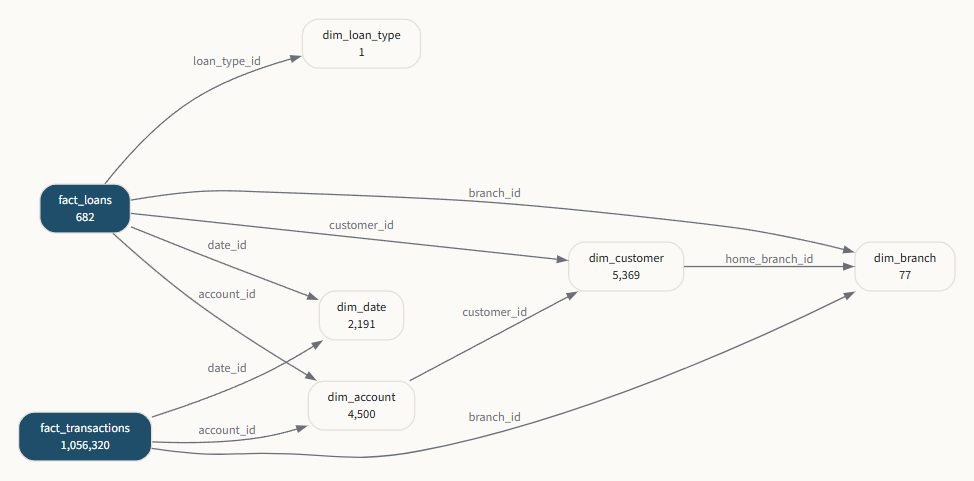
\includegraphics[width=0.9\textwidth]{figures/18_galaxy_schema.png}
    \caption{Generated galaxy-schema diagram used in the dashboard}
    \label{fig:galaxy_png}
\end{figure}

\section{Analytical Queries}
Reporting queries are executed against the modelled tables through the Snowflake reporting views introduced in Chapter~4, and the dashboard performs its own grouped aggregations for its charts. Representative analyses include default rate by branch, monthly transaction totals by type, and balance-based risk quadrants. These queries use ordinary grouping against the conformed dimensions; the focus of this project is the decision-support pipeline rather than a precomputed OLAP cube.

\chapter{Supervised Learning Dataset and Leakage Control}
\section{Dataset Construction}
The supervised task is to predict the binary default label. Each of the 682 loans becomes one row in \texttt{analytics.loan\_features}, a 28-column warehouse table; the exported modelling CSV keeps 27 columns. The target is derived from the loan status: codes B and D (completed unpaid, or running in debt) become \texttt{1}; all other statuses become \texttt{0}. This yields 76 defaults against 606 good loans, an 11.14\% base rate.

\begin{figure}[H]
    \centering
    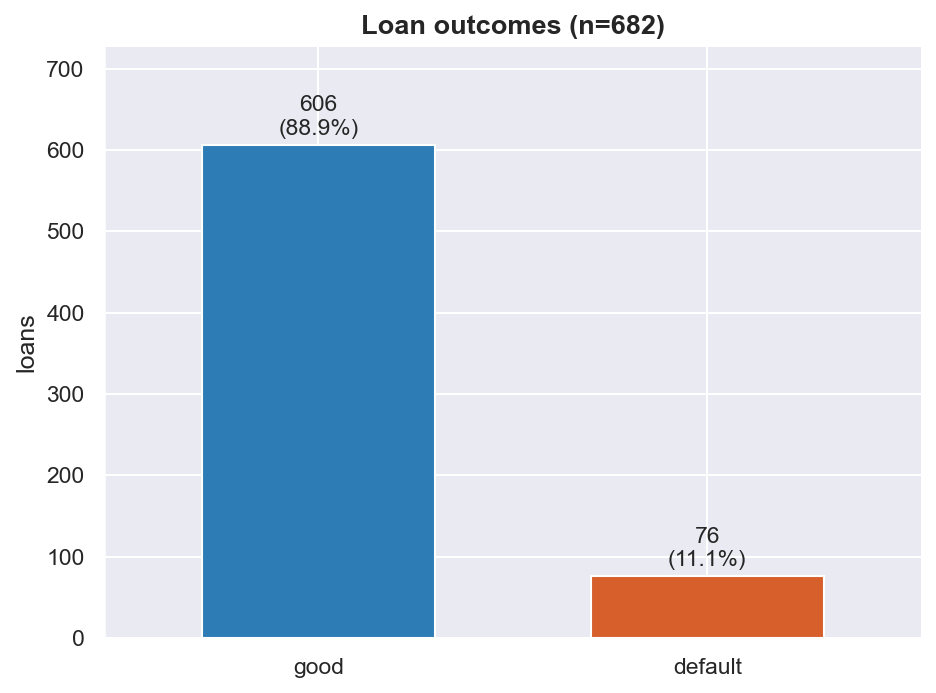
\includegraphics[width=0.9\textwidth]{figures/04_target_distribution.png}
    \caption{Target distribution: 606 good loans and 76 defaults}
    \label{fig:target_distribution}
\end{figure}

\section{Leakage Rule}
The defining constraint is that a feature may only use information available before the loan was granted. The feature query joins each loan to transactions with the condition \texttt{t.date\_id < l.loan\_date\_id}. Strict inequality matters: a transaction on the loan date is excluded. For each loan the aggregation computes transaction counts, turnover, average and standard deviation of amounts, average/minimum/maximum balance, the last balance before the loan, months active, and transaction frequency. All of these come from the pre-loan window.

The build performs an explicit audit: for each feature row it recounts the transactions that satisfy the date condition and compares that count with the stored \texttt{n\_txn}. A mismatch fails the build. The reported result is \texttt{features with post-loan rows: 0}, and the test suite checks the same condition. Figure~\ref{fig:feature_vector} shows how the source tables become one loan feature vector.

\begin{figure}[H]
    \centering
    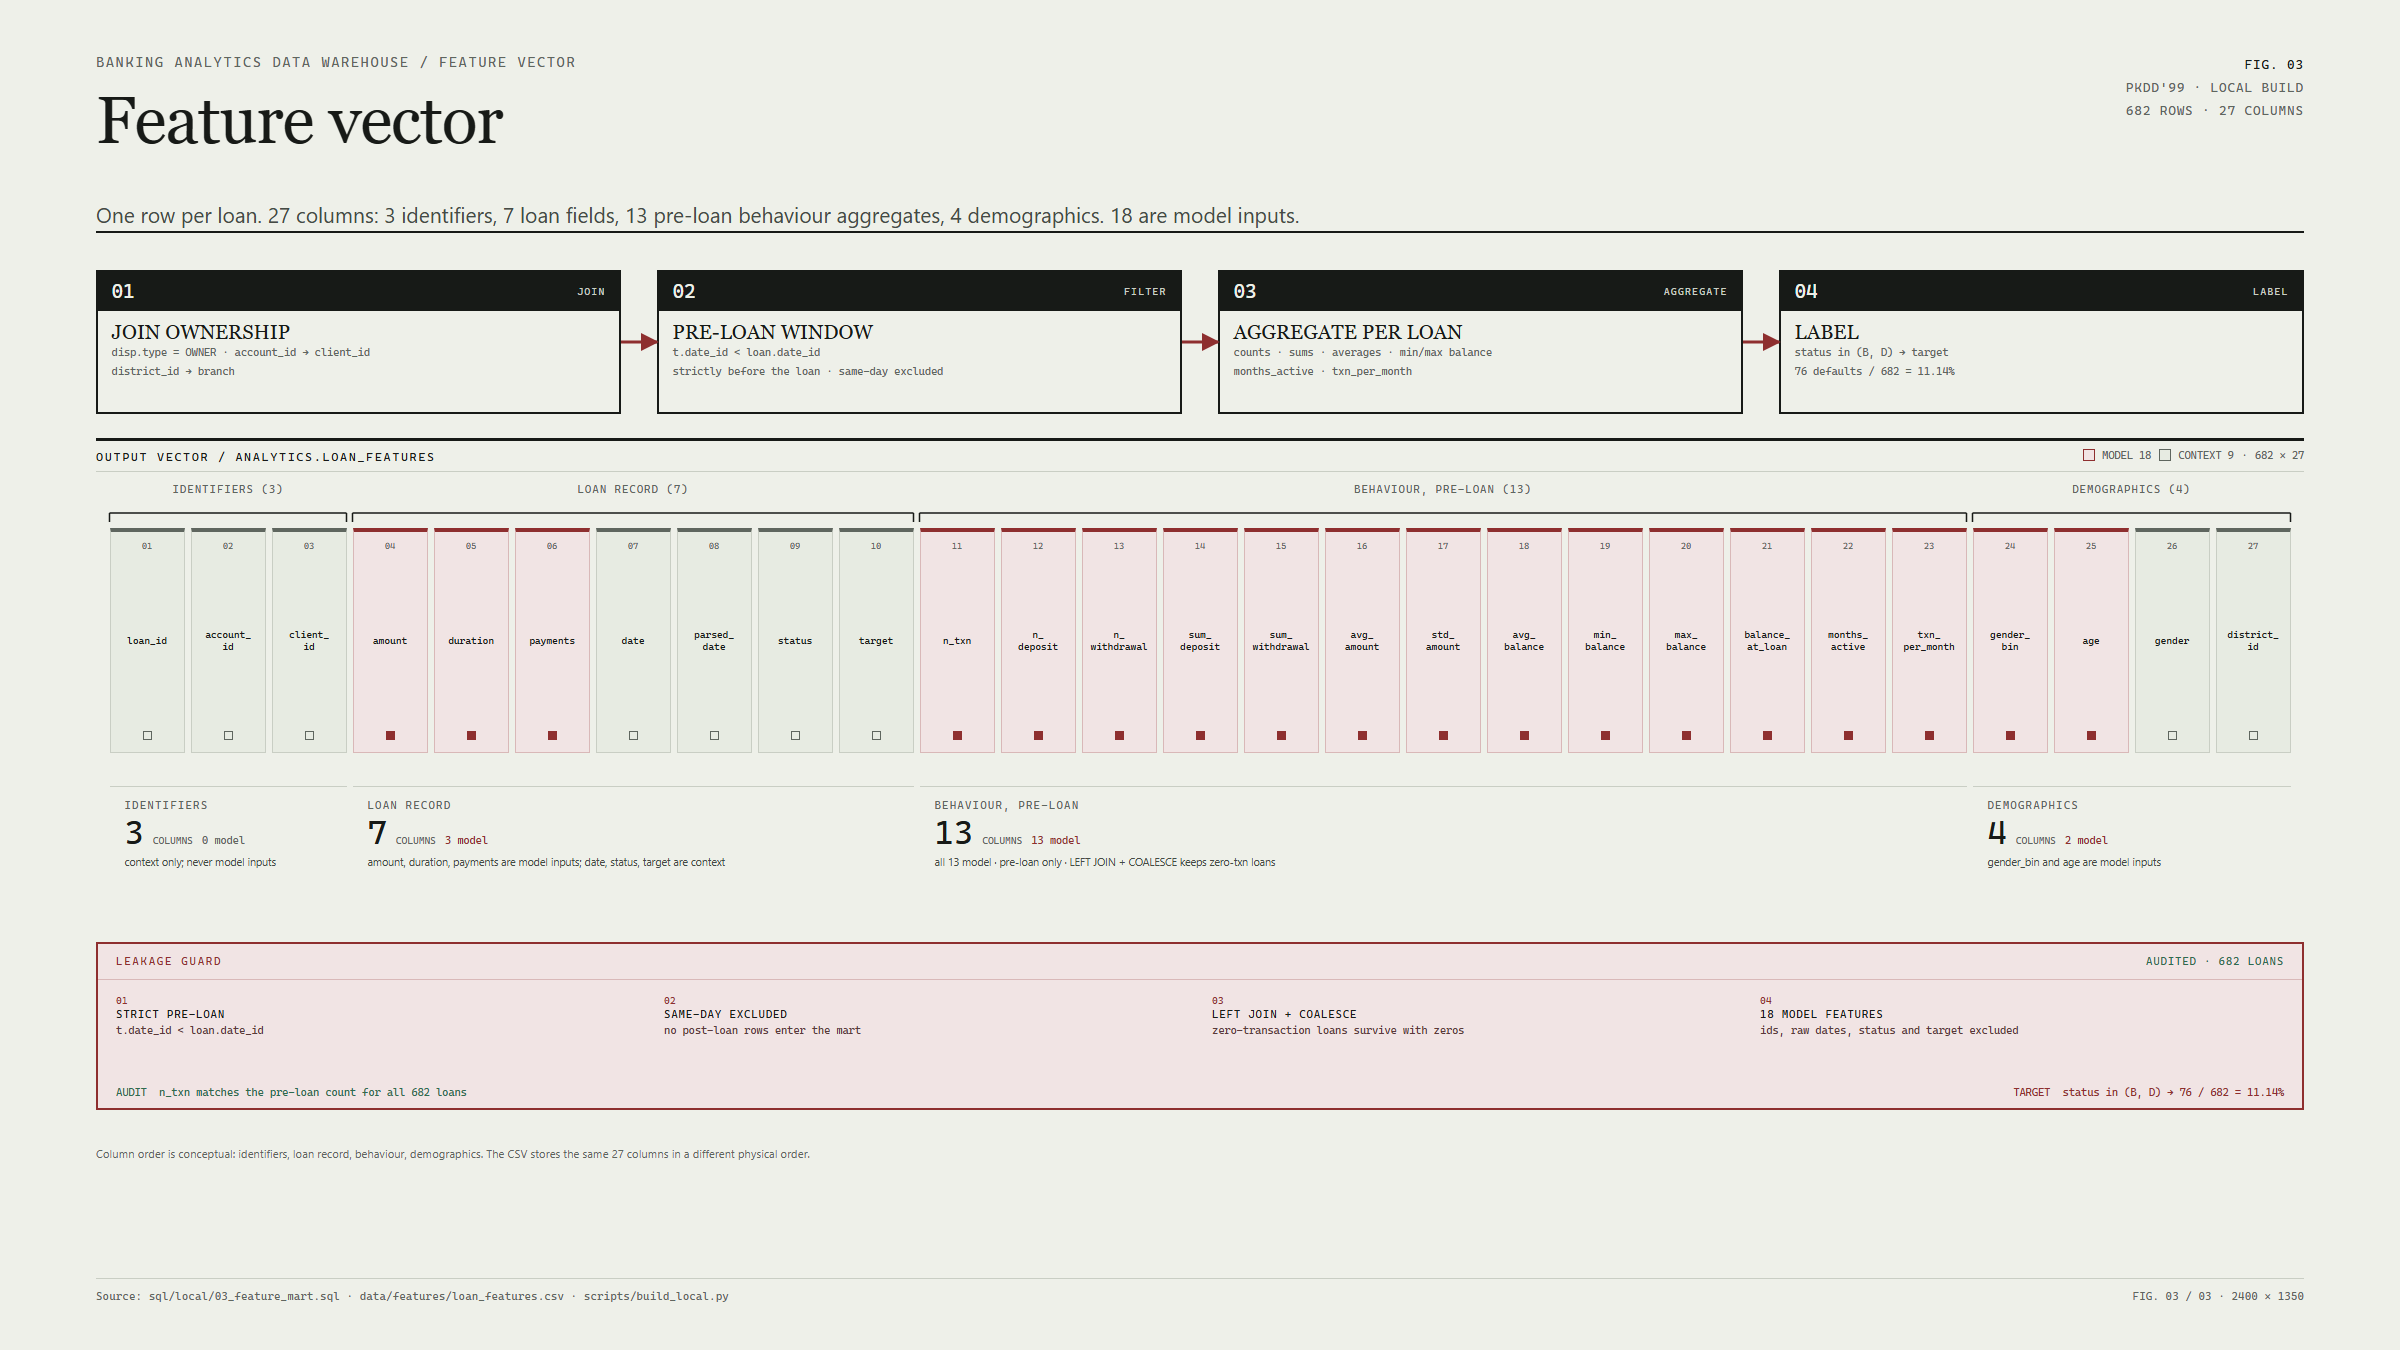
\includegraphics[width=0.9\textwidth]{figures/03_feature_vector.png}
    \caption{From source tables to a leakage-safe loan feature vector}
    \label{fig:feature_vector}
\end{figure}

\section{Feature Set}
Eighteen columns are used as model inputs. They fall into three groups:

\begin{table}[H]
    \centering
    \small
    \renewcommand{\arraystretch}{1.25}
    \begin{tabular}{|l|l|l|}
        \hline
        \textbf{Group} & \textbf{Count} & \textbf{Features} \\
        \hline
        Behavioural & 13 & \texttt{n\_txn}, \texttt{n\_deposit}, \texttt{n\_withdrawal}, \texttt{sum\_deposit}, \texttt{sum\_withdrawal}, \texttt{avg\_amount}, \texttt{std\_amount}, \texttt{avg\_balance}, \texttt{min\_balance}, \texttt{max\_balance}, \texttt{balance\_at\_loan}, \texttt{months\_active}, \texttt{txn\_per\_month} \\
        \hline
        Loan terms & 3 & \texttt{amount}, \texttt{duration}, \texttt{payments} \\
        \hline
        Demographics & 2 & \texttt{age}, \texttt{gender\_bin} \\
        \hline
    \end{tabular}
    \caption{The 18 modelling features}
    \label{tab:feature_groups}
\end{table}

Loan amount, duration, and payments describe the product; age and gender are limited demographics kept as a documented baseline. Behavioural features describe how the account was used before the loan. The unsupervised analysis in Chapter~9 deliberately drops the product and demographic columns and keeps only the 13 behavioural ones.

\section{Exploratory Findings}
The strongest correlations with default are negative balance measures: \texttt{min\_balance} ($-0.26$), \texttt{balance\_at\_loan} ($-0.20$), and \texttt{avg\_balance} ($-0.16$). Loan \texttt{payments} ($+0.18$) and \texttt{amount} ($+0.17$) are the next strongest. Median balance at the loan date is CZK 39,500 for good loans and CZK 22,000 for defaults, while transactions per month are nearly identical (5.7 versus 5.6).

A quadrant at the median balance and median loan amount makes the interaction clearer: the low-balance/high-amount group defaults at 23.3\%, against 4.9\% for high-balance/low-amount. A low balance combined with a large loan is the highest-risk combination, and this agrees with the feature importance reported in Chapter~8.

\section{Preprocessing Boundary}
Scaling, encoding, and oversampling are placed inside the fitted pipeline rather than applied to the whole table. The scaler is fitted on a training fold only, so validation and test folds are not contaminated by their own statistics. SMOTE, when used, is applied inside the training fold as well. This keeps the cross-validation comparison honest and is the second half of the project's leakage control.

\chapter{Pattern Mining}
\section{Basket Construction}
Association-rule mining looks for implications between flags describing an account's behaviour before a loan. The pattern-mining script converts each account's pre-loan transactions into a basket of items: transaction type flags, high-amount activity, negative-balance behaviour, and the observed default outcome. Only transactions strictly before the loan date enter a basket, so the rules obey the same leakage boundary as the supervised features.

\section{Algorithms}
Two algorithms are run over the same baskets:
\begin{itemize}
    \item \textbf{Apriori}, a level-wise candidate-generation method that extends frequent itemsets one item at a time and prunes candidates whose subsets are not frequent.
    \item \textbf{FP-Growth}, which compresses the transactions into a frequent-pattern tree and mines it without generating candidate itemsets.
\end{itemize}

Both are run with minimum support $0.03$ and maximum itemset length $3$. They return the same 41 frequent itemsets, which is a useful consistency check between two different search strategies. The process is summarised in Figure~\ref{fig:pattern_flow}.

\begin{figure}[H]
    \centering
    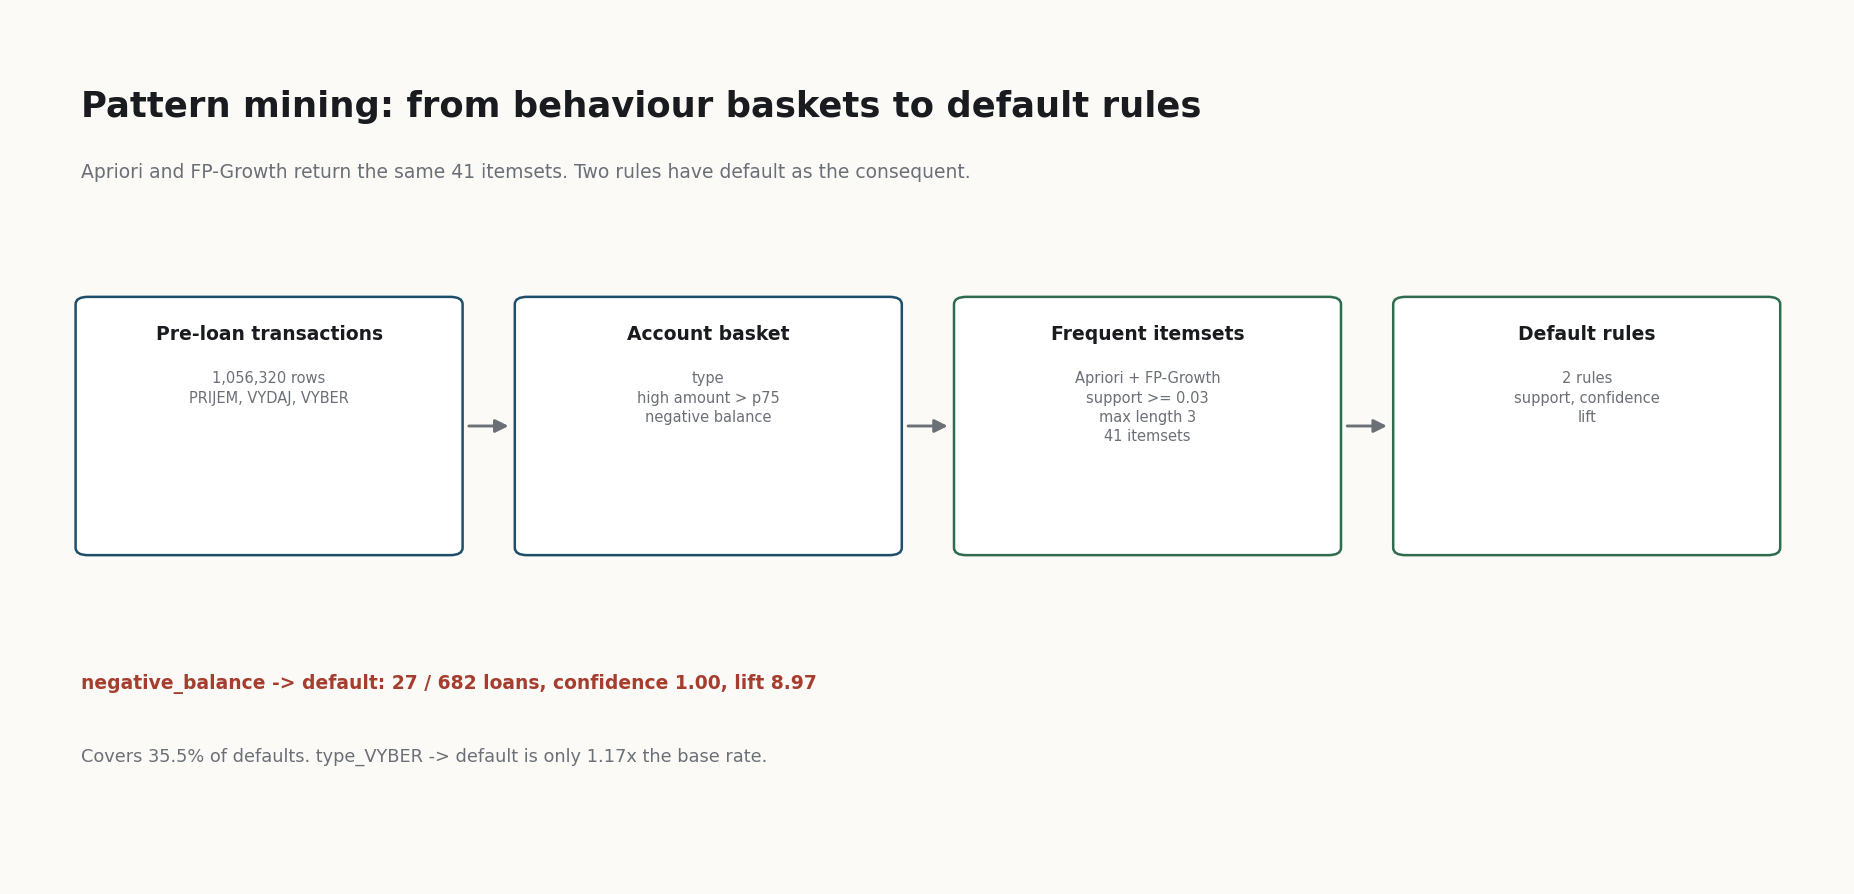
\includegraphics[width=0.88\textwidth]{figures/12_pattern_mining_flow.png}
    \caption{Pattern-mining pipeline from pre-loan baskets to default rules}
    \label{fig:pattern_flow}
\end{figure}

\section{Rules}
Rules are ranked by lift, which measures how much more often the consequent occurs with the antecedent than would be expected from the base rate. Two default-oriented rules survive the support threshold:

\begin{table}[H]
    \centering
    \small
    \renewcommand{\arraystretch}{1.25}
    \begin{tabular}{|l|c|c|c|}
        \hline
        \textbf{Rule} & \textbf{Support} & \textbf{Confidence} & \textbf{Lift} \\
        \hline
        \texttt{negative\_balance $\rightarrow$ default} & 0.0396 (27/682) & 1.000 & 8.97 \\
        \texttt{type\_VYBER $\rightarrow$ default} & 0.0704 (48/682) & 0.130 & 1.17 \\
        \hline
    \end{tabular}
    \caption{Default-oriented association rules}
    \label{tab:rules}
\end{table}

The negative-balance rule covers all 27 loans whose minimum pre-loan balance was negative, all of which defaulted. That is 35.5\% of the 76 defaults, with a lift of 8.97 over the 11.1\% base rate. It is the strongest single finding in the project and agrees with the supervised feature importance, where minimum balance is also the leading input.

The cash-withdrawal rule is only slightly above the base rate, so it is not a useful standalone screen. Its presence mainly confirms that high activity alone does not imply risk.

\section{Interpretation}
The rules are descriptive, not causal. A negative balance does not cause default, but it identifies a group with a much higher observed default rate. In practice the rule can be used as a transparent complement to the model score: a loan that satisfies the negative-balance rule deserves review even if its model score is moderate. The Patterns page of the dashboard shows the rules, itemset support, and rule coverage with covered-loan counts.

\chapter{Classification Models and Validation}
\section{Experimental Setup}
Six classifiers were compared: Decision Tree, Gaussian Naive Bayes, Random Forest (200 trees), Calibrated SVM, K-Nearest Neighbours ($k=5$), and Gradient Boosting. Each was run with and without SMOTE and with default or tuned hyperparameters, giving 24 configurations. Evaluation uses three layers:

\begin{enumerate}
    \item A stratified 75/25 train--test split as a held-out reference.
    \item RandomizedSearchCV with inner 5-fold validation on the training split only.
    \item RepeatedStratifiedKFold with 5 folds and 10 repeats, giving 50 estimates per configuration.
\end{enumerate}

The selection rule is fixed in advance: the highest repeated-CV F1 on the unresampled baseline arm. Fixing the rule before looking at results avoids choosing a model to flatter a preferred metric.

\section{Repeated Cross-Validation Results}
\begin{table}[H]
    \centering
    \small
    \renewcommand{\arraystretch}{1.25}
    \begin{tabular}{|l|l|c|c|c|}
        \hline
        \textbf{Model} & \textbf{Variant} & \textbf{F1} & \textbf{Avg.\ precision} & \textbf{ROC AUC} \\
        \hline
        Gradient Boosting & baseline, tuned & $\mathbf{0.571 \pm 0.120}$ & 0.654 & 0.864 \\
        Decision Tree & baseline, tuned & $0.557 \pm 0.126$ & 0.507 & 0.748 \\
        Random Forest & baseline, tuned & $0.556 \pm 0.112$ & $\mathbf{0.661}$ & $\mathbf{0.877}$ \\
        Random Forest & SMOTE, tuned & 0.542 & 0.638 & 0.872 \\
        Gradient Boosting & SMOTE, tuned & 0.536 & 0.641 & 0.851 \\
        SVM & baseline, tuned & 0.498 & 0.603 & 0.842 \\
        KNN & baseline & 0.223 & 0.249 & 0.628 \\
        \hline
    \end{tabular}
    \caption{Repeated-CV comparison (selected configurations)}
    \label{tab:cv_results}
\end{table}

The top three F1 scores lie within one standard deviation of one another. Random Forest has the best average precision and ROC AUC; Gradient Boosting is selected because it has the highest F1 under the stated rule, not because it dominates every metric. The honest reading is a leading pair rather than a single winner.

\begin{figure}[H]
    \centering
    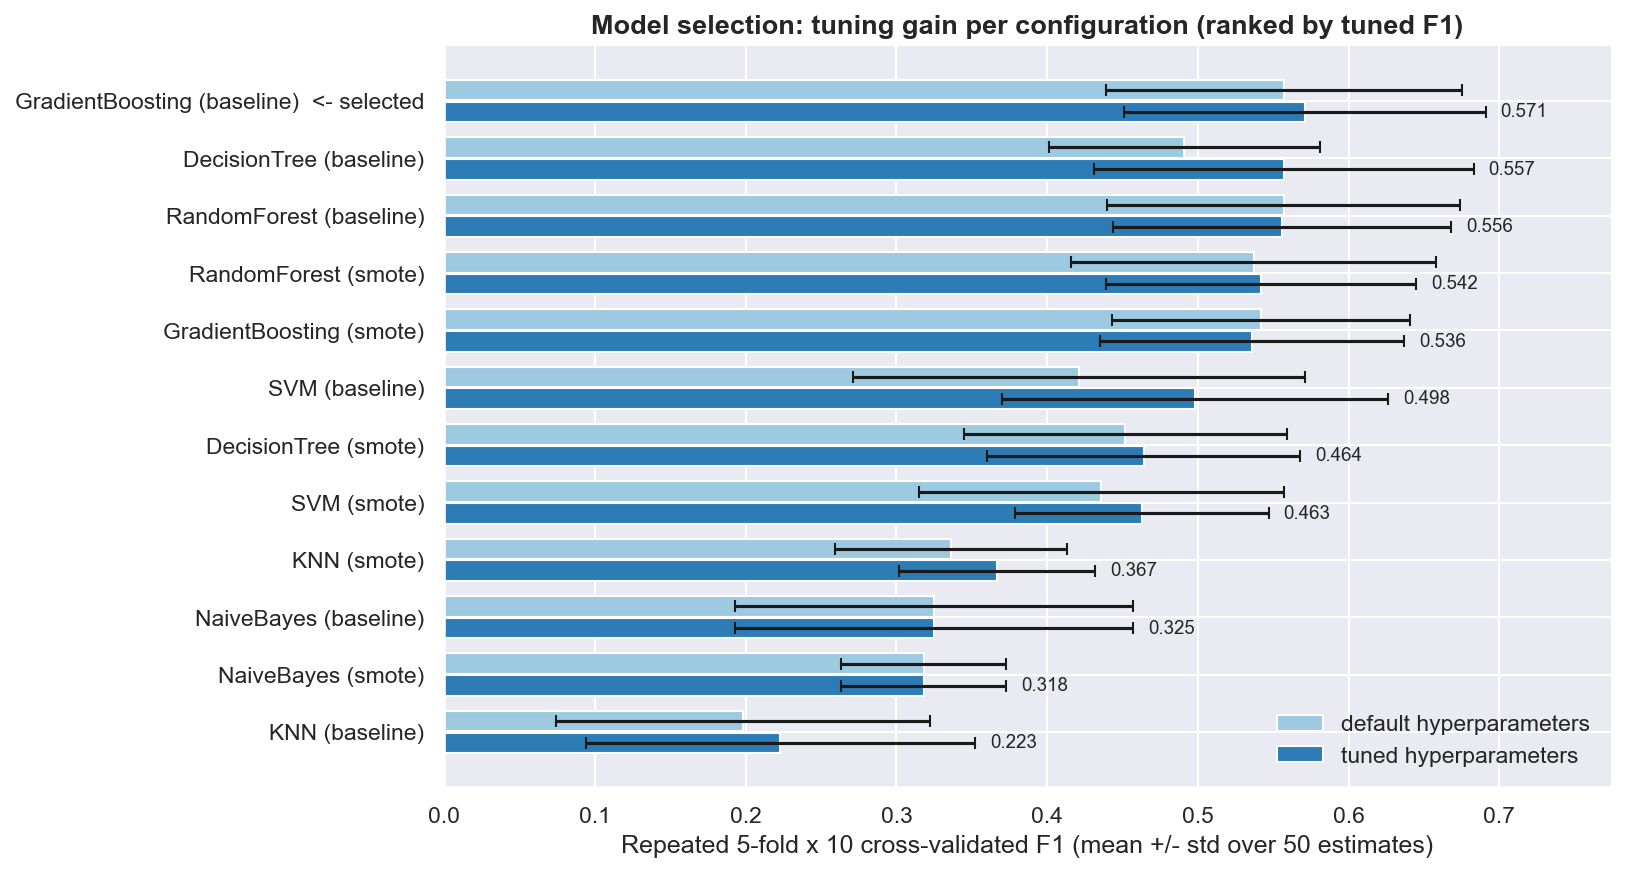
\includegraphics[width=0.9\textwidth]{figures/05_cv_selection.png}
    \caption{Repeated-CV model comparison used for selection}
    \label{fig:cv_selection}
\end{figure}

\section{Threshold-Free Evaluation}
Average precision is the more informative ranking metric here because defaults are rare. The precision--recall curves separate the models less cleanly than the ROC curves, which is expected at an 11\% base rate. Figure~\ref{fig:roc} and Figure~\ref{fig:pr} show the two views, and Figure~\ref{fig:confusion} shows the confusion matrices at the operating points.

\begin{figure}[H]
    \centering
    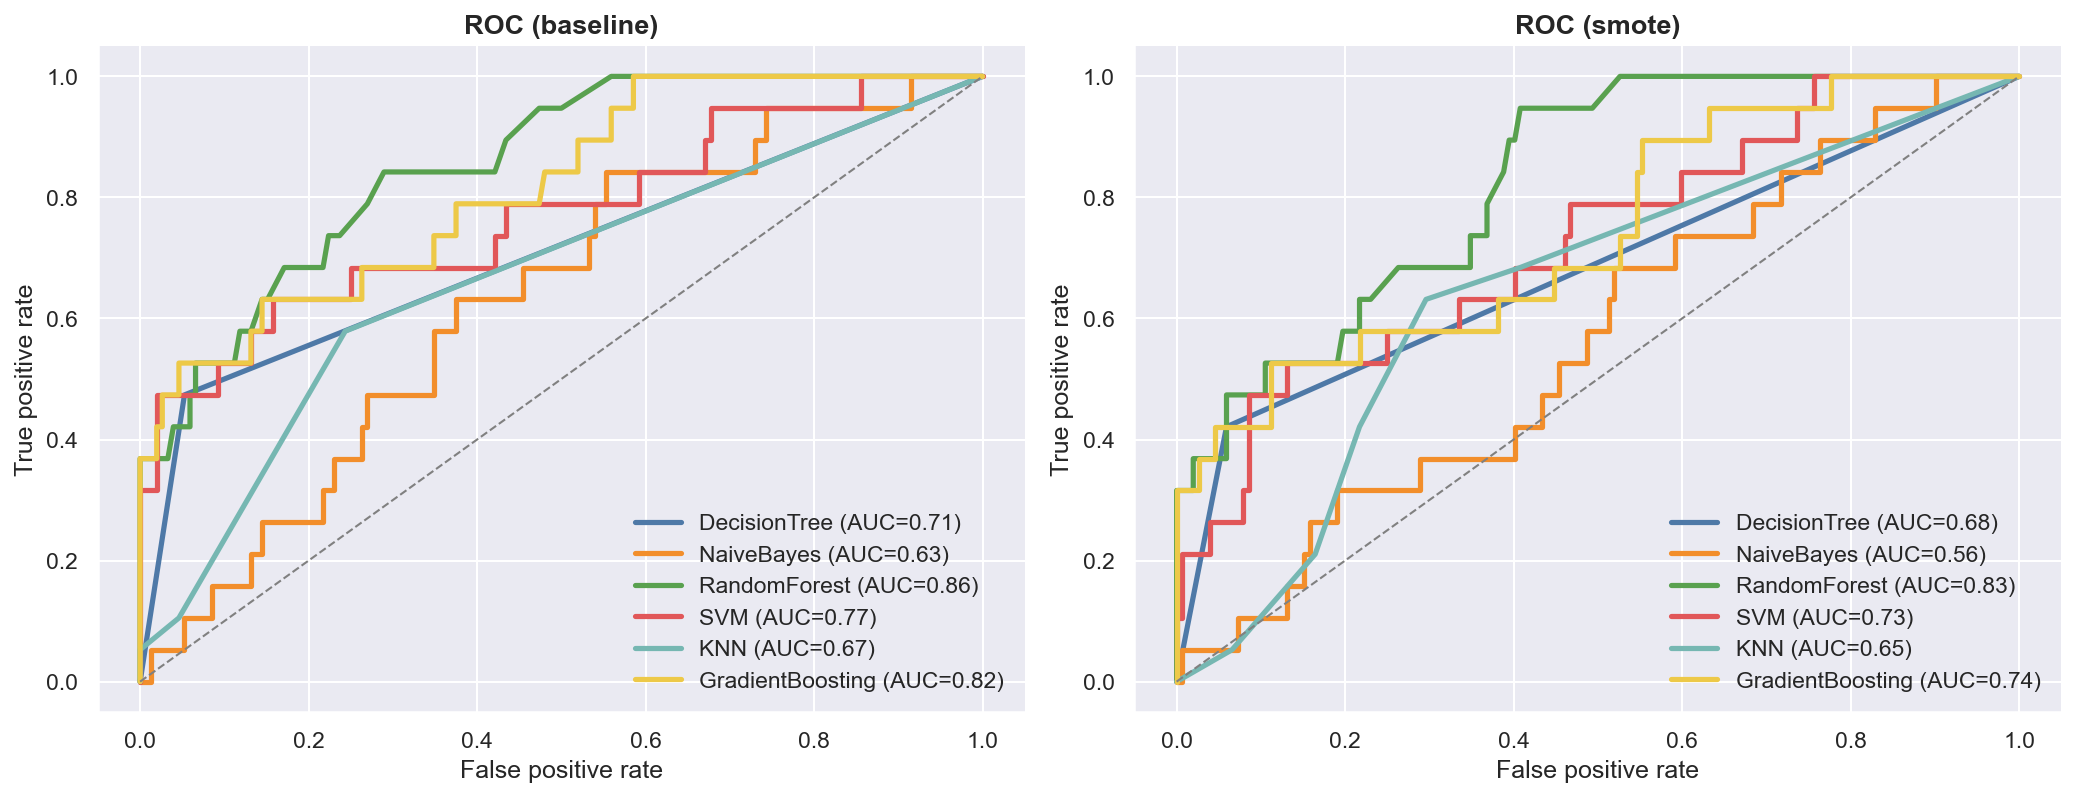
\includegraphics[width=0.85\textwidth]{figures/06_roc_curves.png}
    \caption{ROC curves for the compared classifiers}
    \label{fig:roc}
\end{figure}

\begin{figure}[H]
    \centering
    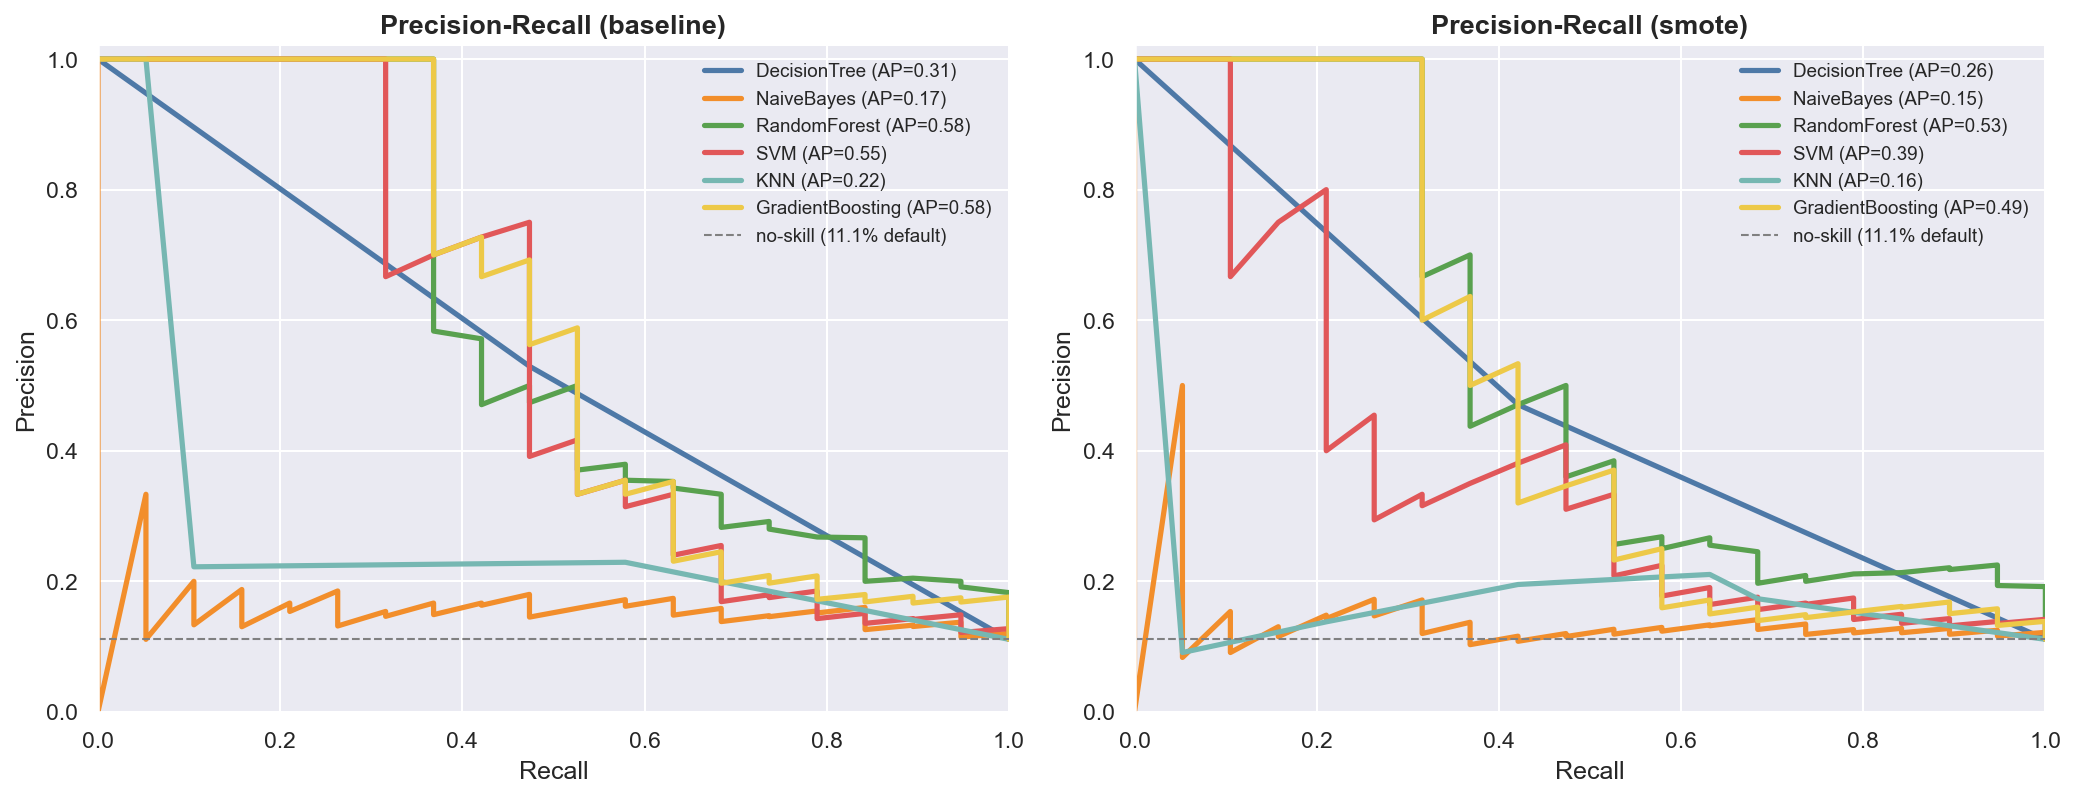
\includegraphics[width=0.85\textwidth]{figures/07_pr_curves.png}
    \caption{Precision--recall curves for the compared classifiers}
    \label{fig:pr}
\end{figure}

\begin{figure}[H]
    \centering
    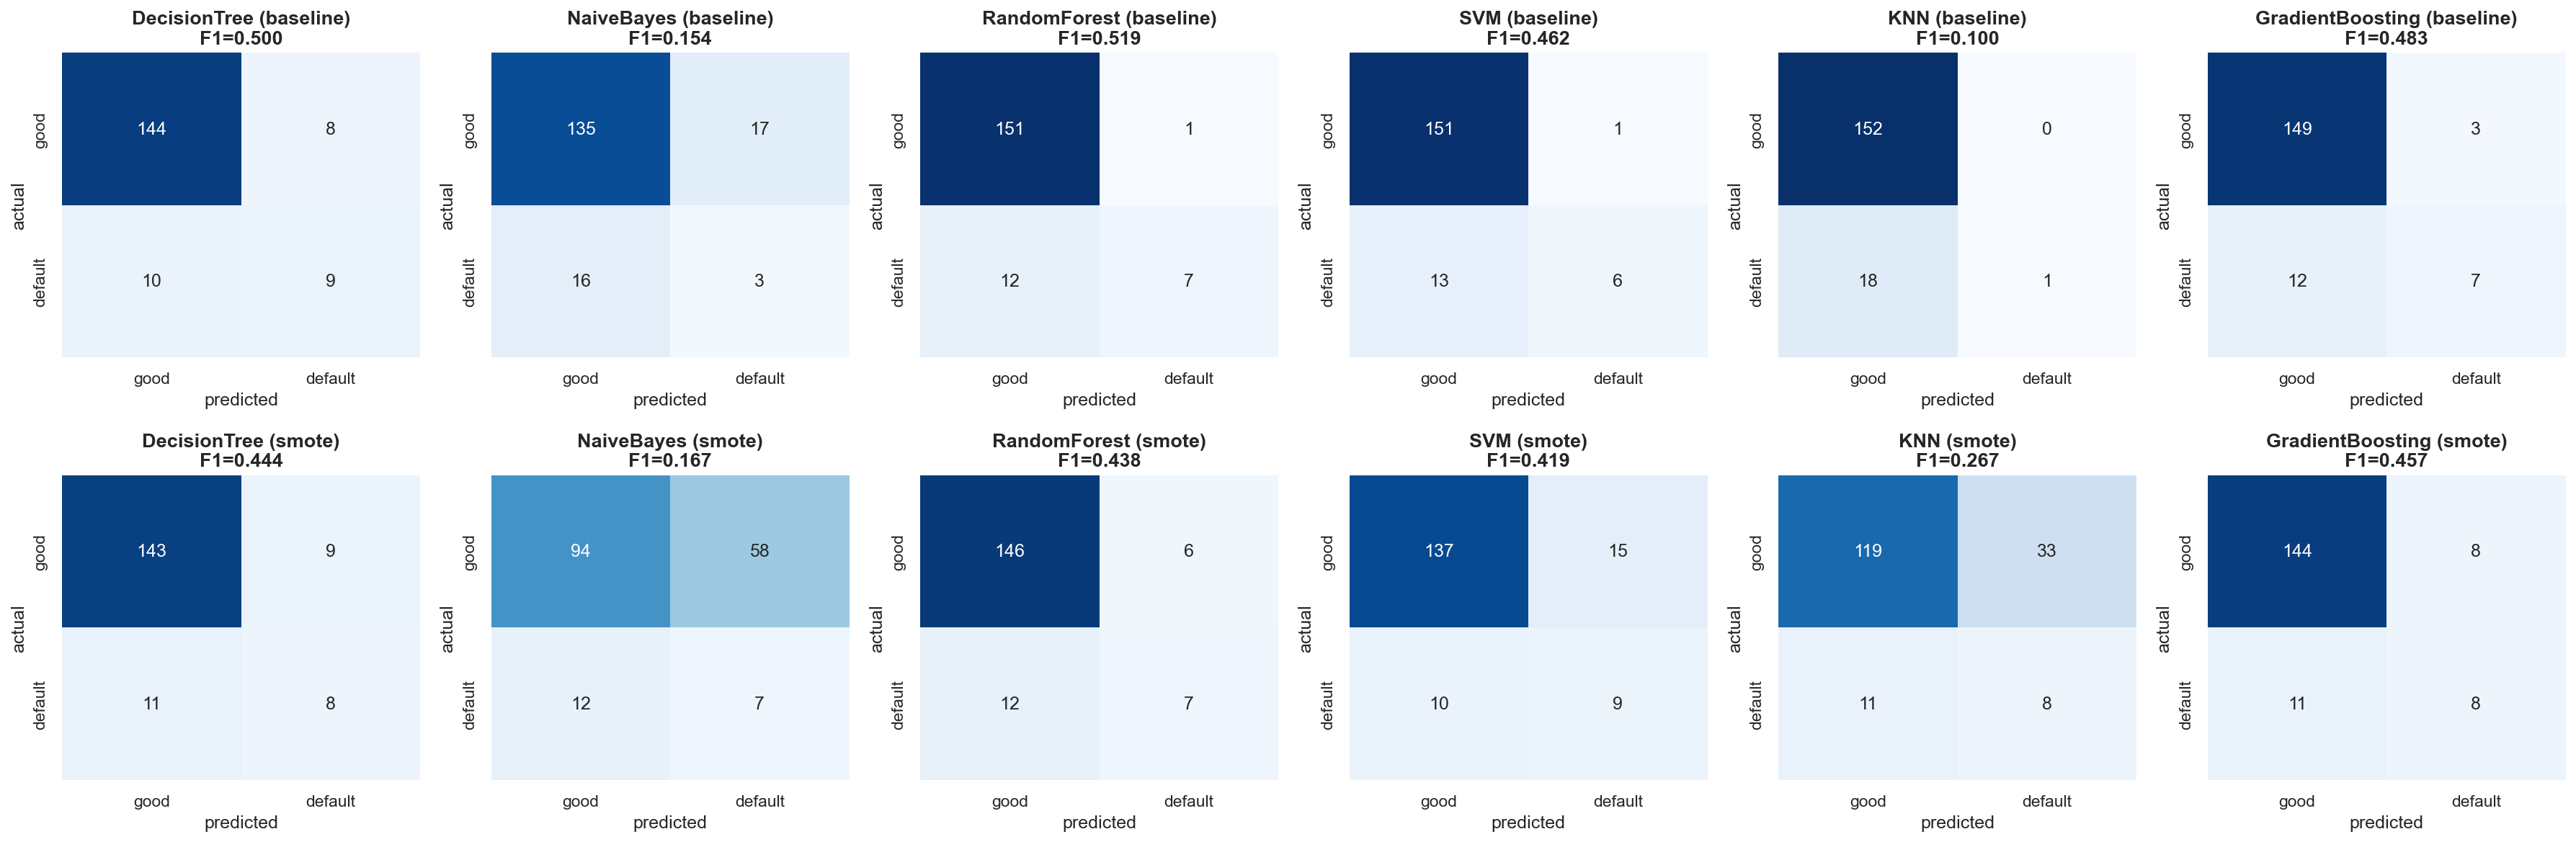
\includegraphics[width=0.88\textwidth]{figures/08_confusion_matrices.png}
    \caption{Confusion matrices at the reported operating points}
    \label{fig:confusion}
\end{figure}

\section{What the Comparison Shows}
\begin{itemize}
    \item SMOTE lowers F1 for five of the six models. It helps KNN, but KNN remains the weakest model.
    \item Hyperparameter tuning materially helps SVM ($+0.077$ F1) and Decision Tree ($+0.066$ F1).
    \item The ensemble models are relatively stable under tuning.
    \item With only 76 defaults, differences below roughly $0.05$ F1 are inside the observed fold-to-fold spread.
\end{itemize}

\begin{figure}[H]
    \centering
    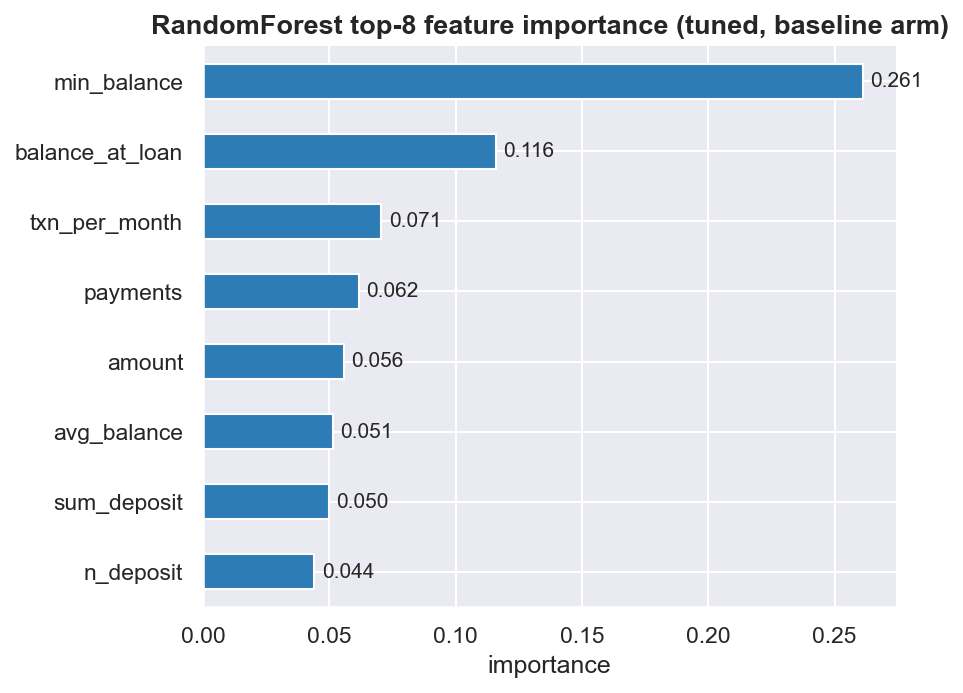
\includegraphics[width=0.85\textwidth]{figures/09_feature_importance.png}
    \caption{Random Forest feature importance}
    \label{fig:importance}
\end{figure}

Random Forest importance agrees with the correlations in Chapter~6: \texttt{min\_balance} leads, followed by \texttt{balance\_at\_loan}, transaction frequency, payments, and amount. Age and gender are close to zero.

\section{Performance Metrics}
The reported classification metrics are defined as follows, with $TP$, $FP$, and $FN$ taken from the confusion matrix:

\begin{itemize}
    \item \textbf{Accuracy:} $(TP + TN) / (TP + TN + FP + FN)$. Limited use here because of class imbalance.
    \item \textbf{Precision:} $TP / (TP + FP)$, the share of flagged loans that actually default.
    \item \textbf{Recall:} $TP / (TP + FN)$, the share of defaults caught.
    \item \textbf{F1:} the harmonic mean of precision and recall; the selection metric.
    \item \textbf{Average precision:} area under the precision--recall curve, more informative than ROC AUC at low base rates.
    \item \textbf{ROC AUC:} probability that a random default scores above a random non-default.
\end{itemize}

All classification metrics come from out-of-fold scores and the held-out split. Clustering metrics, which are internal and do not use the default label, are reported separately in Chapter~9.

\section{Selected Model Implementation}
The tuned Gradient Boosting pipeline is saved with preprocessing included, so a new application is transformed with exactly the same steps used in training. Two challengers were also trained and saved: an MLP neural network and a classification-rule learner (CBA).

\begin{table}[H]
    \centering
    \small
    \begin{tabular}{|l|c|c|c|c|}
        \hline
        \textbf{Model} & \textbf{Precision} & \textbf{Recall} & \textbf{F1} & \textbf{ROC AUC} \\
        \hline
        MLP & 0.694 & 0.329 & 0.446 & 0.750 \\
        CBA rules & $\mathbf{1.000}$ & 0.355 & 0.524 & 0.678 \\
        \hline
    \end{tabular}
    \caption{Additional models}
    \label{tab:additional_models}
\end{table}

The CBA rules are precise but catch only about one third of defaults, and all of them key off a negative minimum balance. That matches both the rule mining and the feature importance. The Simulator page of the dashboard loads the saved Gradient Boosting pipeline, scores one application, places it against the portfolio score distribution, and reports one-at-a-time stress drivers. No model is retrained when the dashboard starts.

\chapter{Unsupervised Learning and Clustering}
\section{Purpose}
The supervised model answers ``is this loan likely to default?''. Clustering answers a different question: ``are there natural groups of borrowing behaviour in the portfolio?''. The default label is never used to fit or select clusters; it is joined back afterwards only to describe the groups. This keeps the segmentation an unsupervised result.

\section{Unsupervised Dataset}
The same 682 loans are used, but with a different view: only the 13 pre-loan behavioural features from Chapter~6. Loan amount, duration, and payments are excluded because they describe the product, not behaviour. Age and gender are excluded because they are demographic attributes and should not drive segmentation. The matrix has no missing values and no zero-variance columns, and a Hopkins statistic of about $0.85$ indicates real clusterable structure.

Several features are correlated: deposit and withdrawal value correlate at $0.997$, transaction count and withdrawal count at $0.981$, and average and standard deviation of amount at $0.941$. Features are standardised with \texttt{StandardScaler}. PCA is used only for two-dimensional visualisation, never for fitting. A pruned six-feature sensitivity set raises silhouette slightly, but the 13-feature set is kept as the primary view because it covers both activity volume and balance behaviour.

\section{Selection Rule}
All four algorithms use the same 682 $\times$ 13 standardised matrix and the same rule: no target, minimum cluster share of 5\%, and the highest valid silhouette. K-Means and K-Medoids search $k=2\ldots6$; AGNES uses Ward linkage over the same range; DBSCAN scans $\epsilon = 0.8\ldots2.0$ with \texttt{min\_samples = 5}. Stability is the mean Adjusted Rand Index over 10 subsamples of 90\% of the loans.

\section{Four-Algorithm Comparison}
\begin{table}[H]
    \centering
    \small
    \renewcommand{\arraystretch}{1.25}
    \resizebox{\textwidth}{!}{
    \begin{tabular}{|l|c|c|c|c|c|c|}
        \hline
        \textbf{Algorithm} & \textbf{Settings} & \textbf{Sizes} & \textbf{Default rate} & \textbf{Silhouette} & \textbf{Davies--Bouldin} & \textbf{Stability ARI} \\
        \hline
        K-Means & $k=2$, $n\_init=10$ & 421 / 261 & 12.35\% / 9.20\% & 0.294 & 1.346 & $0.931 \pm 0.095$ \\
        K-Medoids & $k=2$, 5 restarts & 386 / 296 & 12.18\% / 9.80\% & 0.282 & 1.406 & $0.534 \pm 0.202$ \\
        AGNES & Ward, $k=2$ & 568 / 114 & 11.80\% / 7.89\% & 0.288 & 1.219 & $0.421 \pm 0.148$ \\
        DBSCAN & $\epsilon=1.4$, 5 samples & 553 / 129 & 8.32\% / 23.26\% & n/a & n/a & $0.847 \pm 0.106$ \\
        \hline
    \end{tabular}
    }
    \caption{Clustering comparison on the same 13-feature matrix}
    \label{tab:clustering_compare}
\end{table}

DBSCAN could not produce two stable clusters of at least 5\% each at a reasonable noise level: its second groups contained only 3--21 loans, so they were merged into noise. The selected solution is one dense core plus an outlier layer. Silhouette, Davies--Bouldin, and Calinski--Harabasz are undefined for one cluster and are shown as n/a. Calinski--Harabasz values for the three two-cluster solutions are 306.3, 285.0, and 200.2 for K-Means, K-Medoids, and AGNES respectively.

\begin{figure}[H]
    \centering
    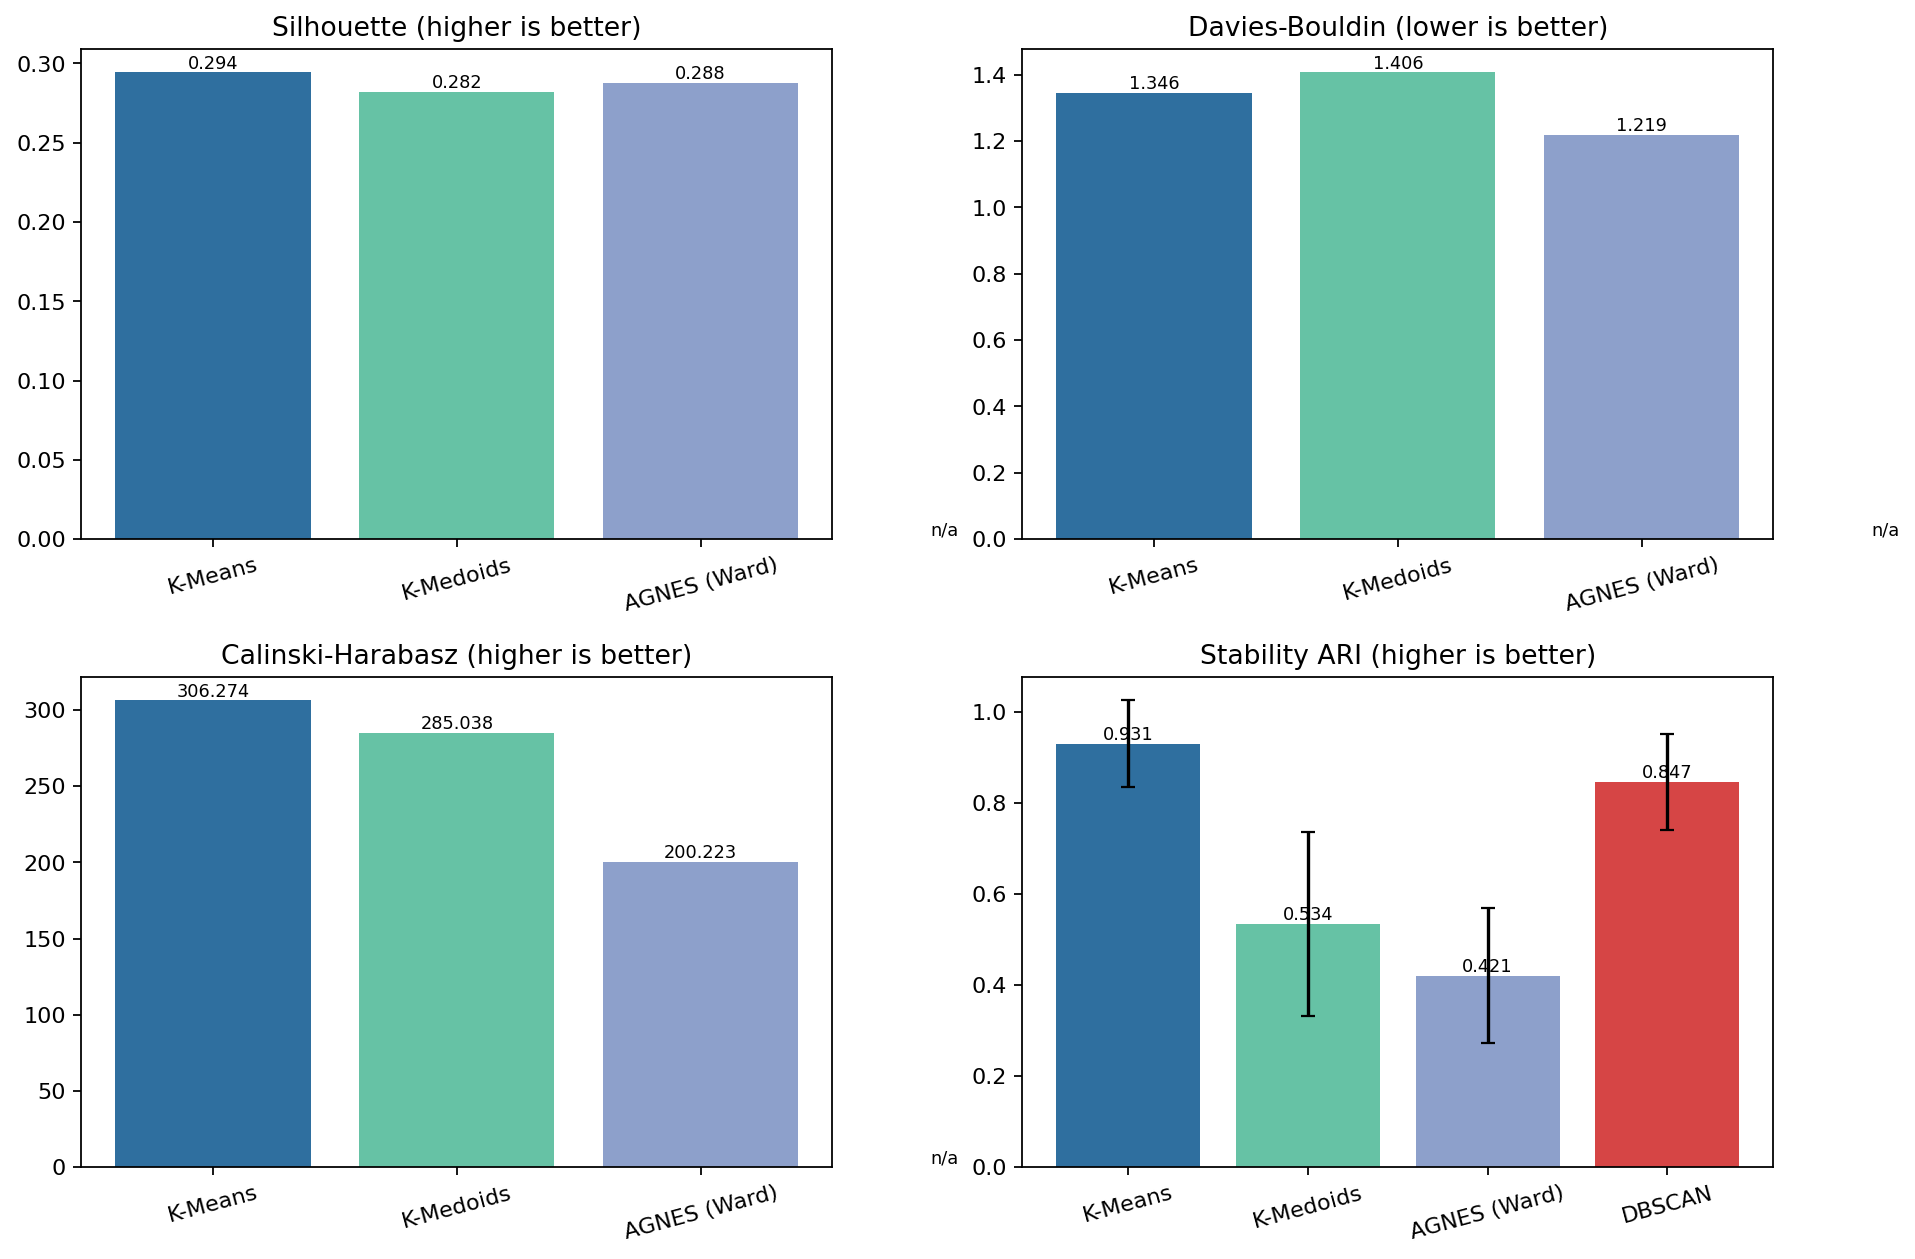
\includegraphics[width=0.88\textwidth]{figures/23_clustering_metrics.png}
    \caption{Internal clustering metric comparison}
    \label{fig:clustering_metrics}
\end{figure}

\begin{figure}[H]
    \centering
    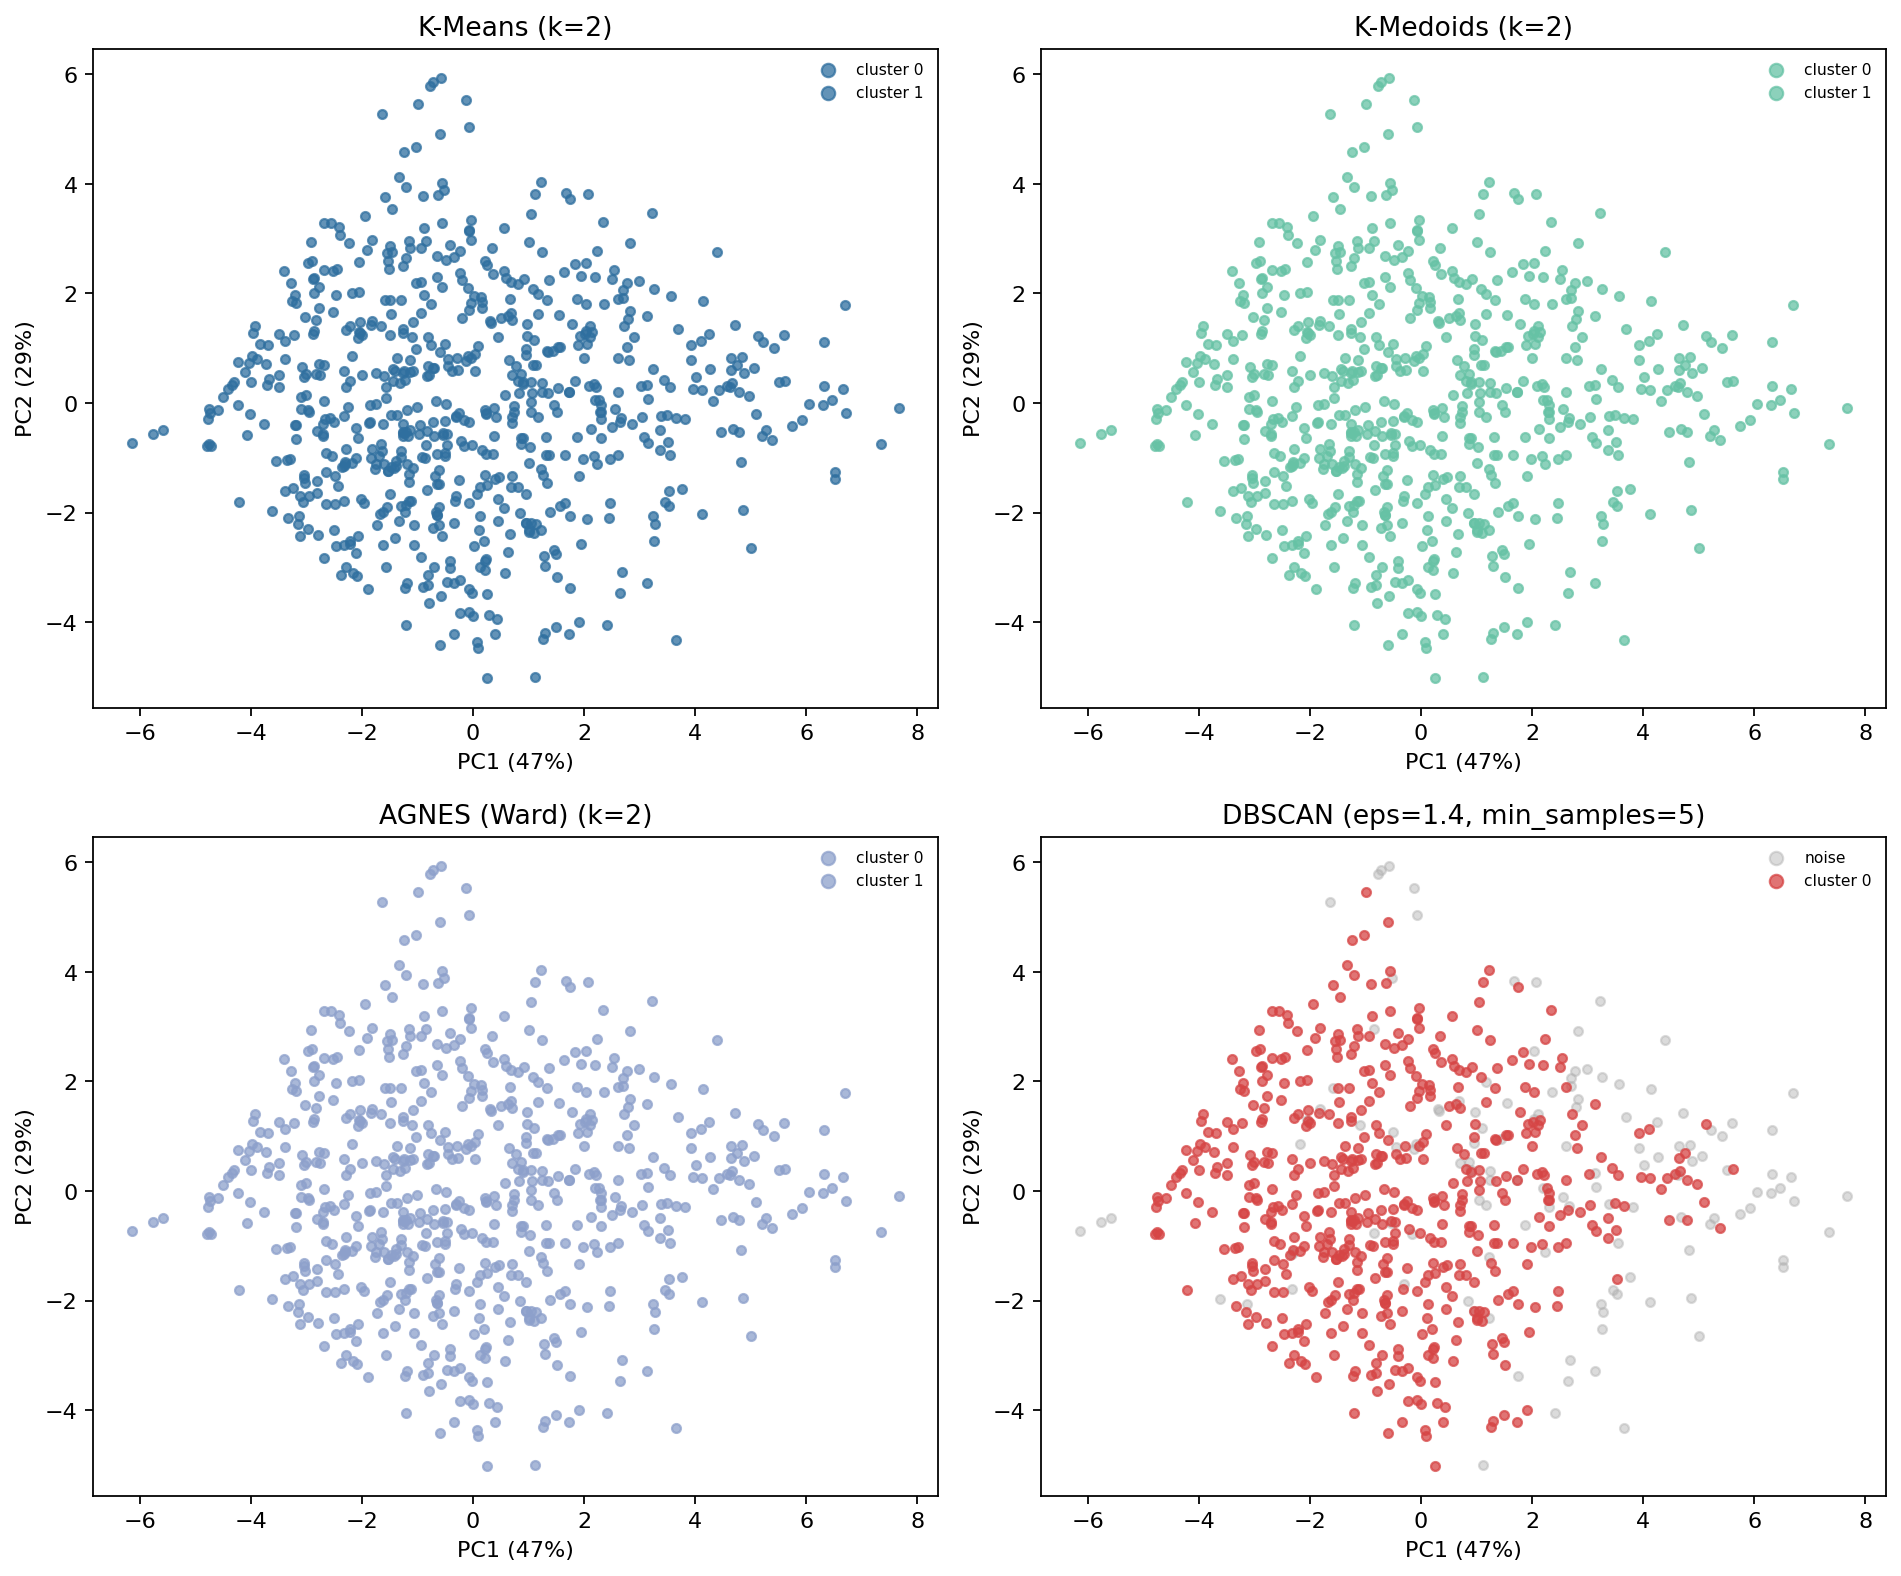
\includegraphics[width=0.88\textwidth]{figures/24_clustering_pca.png}
    \caption{PCA maps of the four clustering solutions}
    \label{fig:clustering_pca}
\end{figure}

\section{Strengths and Limitations}
\begin{itemize}
    \item \textbf{K-Means:} fast, stable, full coverage, and able to score new loans. It assumes roughly spherical, similarly sized clusters and needs $k$. Recommended as the primary method.
    \item \textbf{K-Medoids:} robust to outliers and medoids are real loans, but it is initialisation-sensitive, slower, and much less stable here (ARI $0.534$).
    \item \textbf{AGNES:} builds a hierarchy with no centroid assumption, but has no natural predict step and is the least stable of the three two-cluster methods.
    \item \textbf{DBSCAN:} finds arbitrary shapes and isolates noise, but on this data produces one dense core only. Its value is as an outlier and risk flag.
\end{itemize}

Gaussian Mixture Models were also tested but left out of the main table because BIC and silhouette disagreed on the number of components. The rubric requires a minimum of four algorithms, which the table satisfies.

\section{Selected Implementation}
K-Means with $k=2$ separates a larger low-activity group (421 loans, 52 defaults, 12.35\%) from a smaller high-activity group (261 loans, 24 defaults, 9.20\%). The low-activity group has a median of about 54 transactions, 10 months active, and a CZK 37{,}000 average balance; the high-activity group has about 116 transactions, 17 months active, and a CZK 52{,}000 average balance. The separation is modest, so the segments are broad tendencies rather than distinct customer types.

The implementation is held in the model-building script, which defines the feature list and the selection functions for the partitional and density-based methods. The choice of $k=2$ is supported by silhouette and elbow plots in the segmentation notebook. Outputs include cluster labels, cluster profiles, and loan segments saved under the \texttt{artifacts} directory.

\section{Practical Meaning}
The segment should be combined with the supervised score, not used instead of it. Low-activity loans can enter an earlier engagement or reminder queue; high-activity loans can follow standard monitoring. DBSCAN noise is a separate manual-review flag: 129 loans, 30 defaults, 23.26\% default rate, more than twice the 11.14\% base rate. The labels are descriptive, not causal, and should not become automatic rejection rules.

\begin{figure}[H]
    \centering
    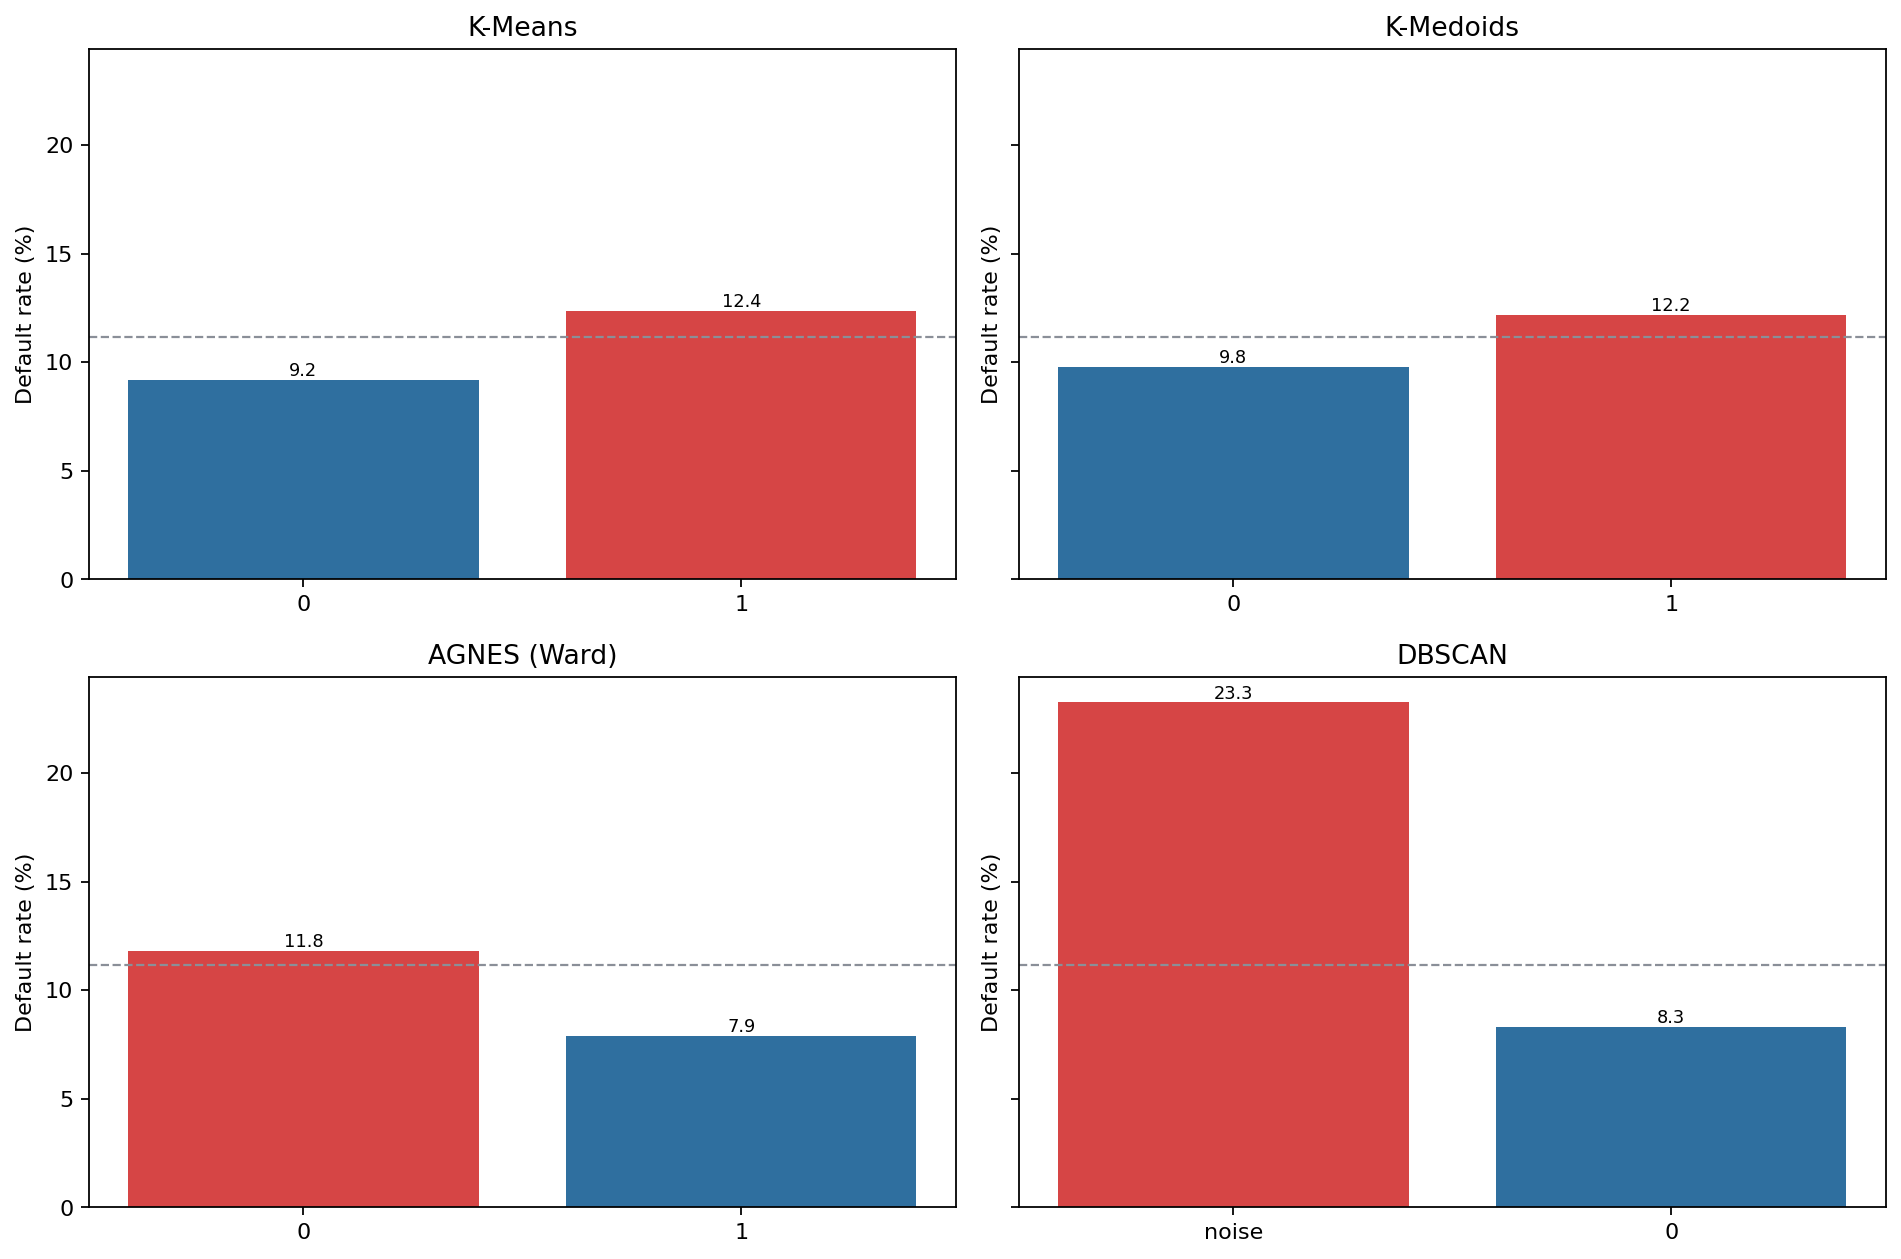
\includegraphics[width=0.88\textwidth]{figures/25_clustering_default_rates.png}
    \caption{Observed default rate by cluster}
    \label{fig:cluster_rates}
\end{figure}

\section{Clustering Metrics}
Silhouette (higher is better) compares within-cluster cohesion with separation to the nearest other cluster. Davies--Bouldin (lower is better) averages the worst pairwise cluster similarity. Calinski--Harabasz (higher is better) is the ratio of between-cluster to within-cluster dispersion. Adjusted Rand Index (higher is better) measures agreement between clusterings on subsamples and is invariant to label permutation.

None of these metrics uses the target. Accuracy, precision, recall, F1, and the confusion matrix belong to the supervised classification in Chapter~8; applying them to clusters would require treating an arbitrary cluster label as a class and would be misleading.

\chapter{Results and Visualizations}
The previous chapters described the warehouse, the models, the mined rules, and the segments. This chapter shows how those results are delivered to a jury or a review analyst. All results are presented through one eight-page Streamlit application rather than a set of static reports.

\section{Dashboard Architecture}
The dashboard is an eight-page Streamlit app. In the reported deployment it reads the six modelled MART tables directly from Snowflake; this is selected by setting the environment variable \texttt{DATA\_SOURCE=snowflake}. Saved artifacts in the \texttt{artifacts} directory supply the model pipelines, scores, rule sets, and cluster labels. The app never retrains a model on page load, so opening a page reproduces exactly the numbers reported in this document.

Every chart is built with Altair, which gives hover tooltips, zoom, and pan on all plots. The schema drawing on the data model card uses Graphviz. The layout follows the same colour palette as the figures in this report: magenta for the primary series, teal for the secondary series, and amber for accents.

\section{Executive Overview}
\begin{figure}[H]
    \centering
    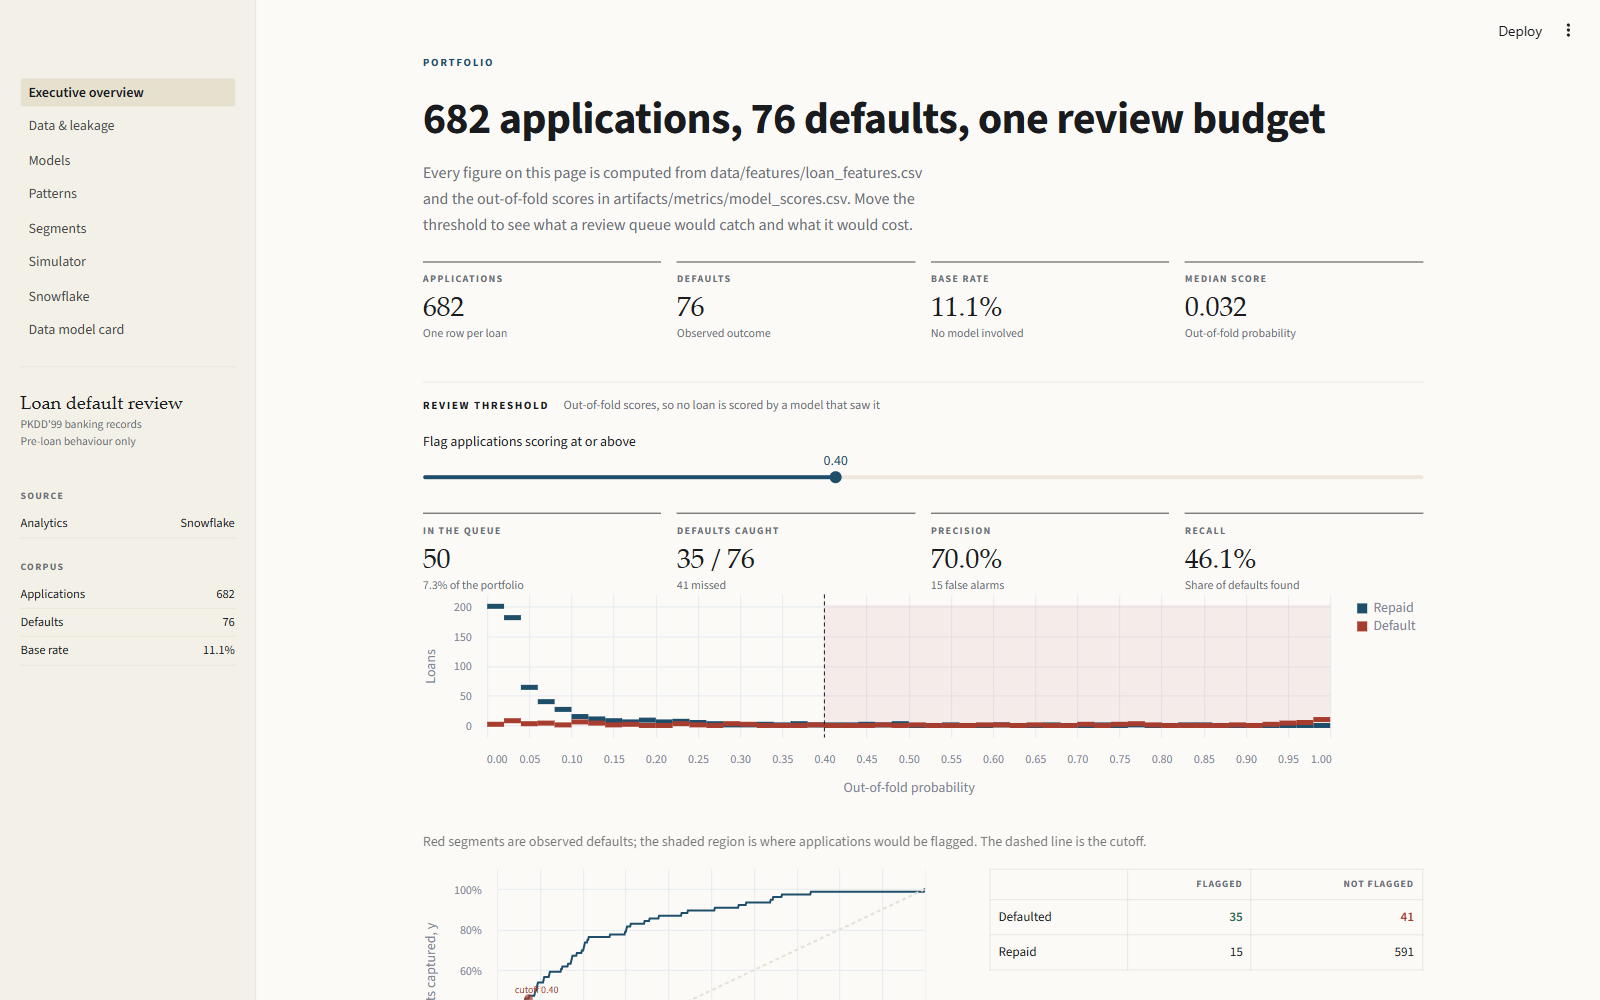
\includegraphics[width=0.92\textwidth]{figures/13_dashboard_executive.png}
    \caption{Executive overview page of the Streamlit dashboard}
    \label{fig:dashboard_executive}
\end{figure}

The executive page is the landing view. A cutoff slider drives the whole page: moving it recomputes the confusion matrix, the exposure figure, and the operating-point metrics from the saved scores. A stacked score histogram shows how defaults and non-defaults distribute across the score range, and a cumulative gains curve shows what share of defaults is captured by reviewing the top-ranked share of the portfolio. A precision/recall trade-off is drawn from a 5\% to 90\% cutoff, and quintile default rates are plotted against the 11.14\% base rate so the lift of ranking is visible at a glance. A segment scatter places loans by their behavioural position, and the selected model's confusion matrix is shown at the current cutoff.

\section{Data and Leakage Page}
\begin{figure}[H]
    \centering
    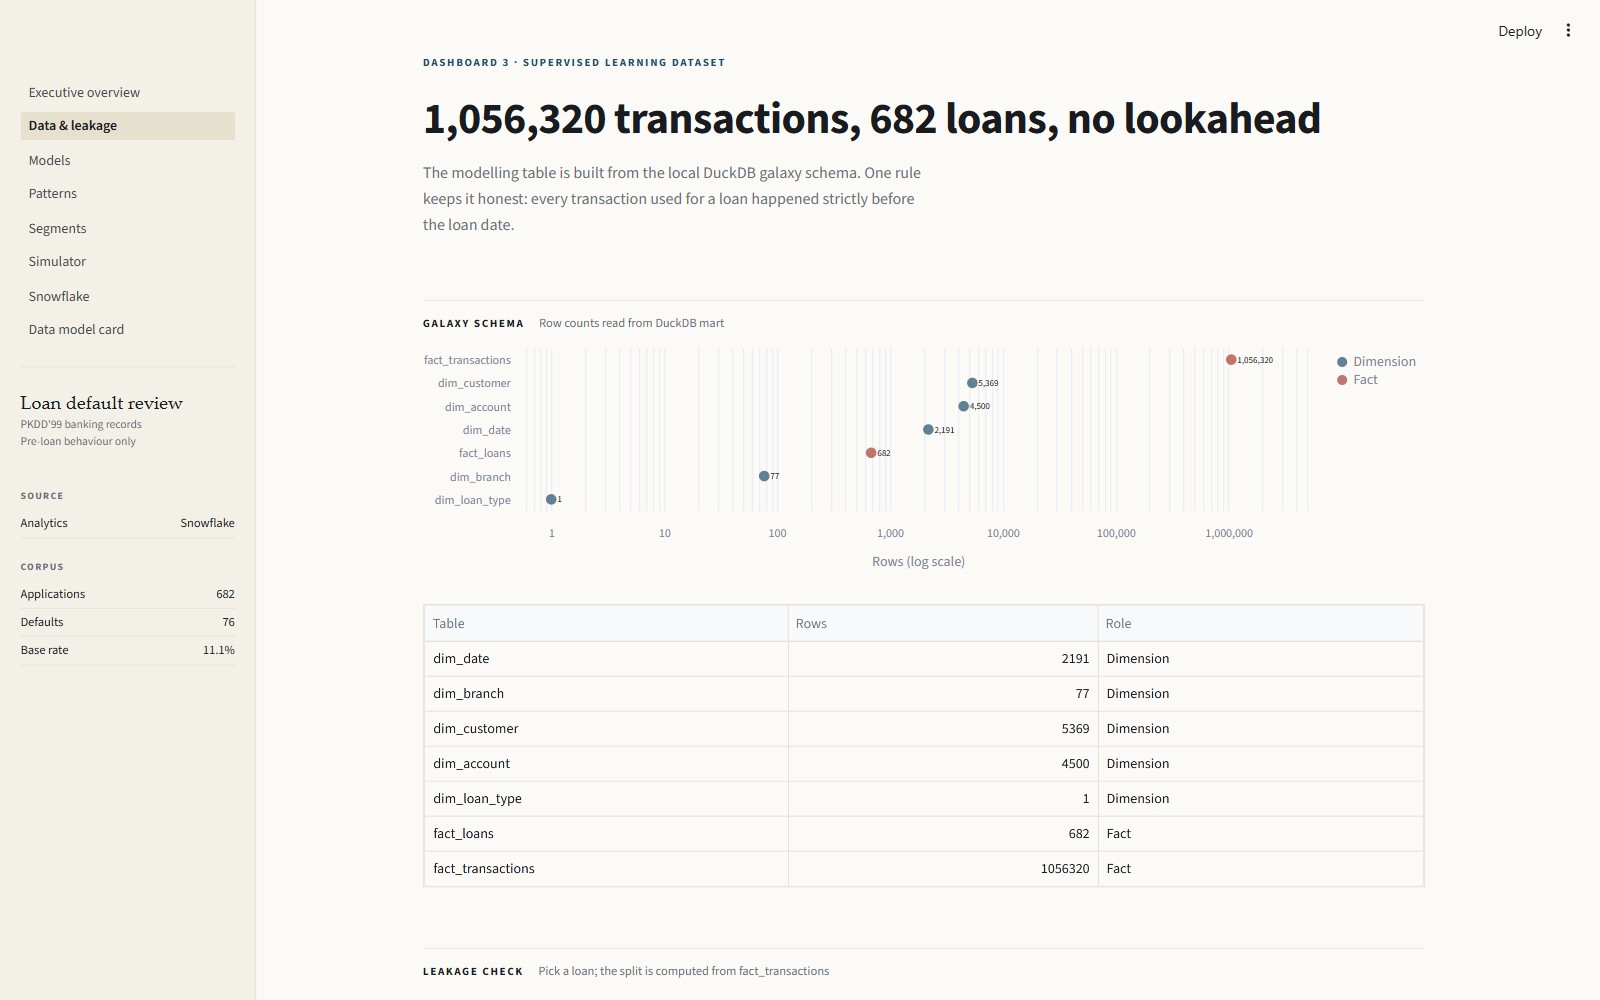
\includegraphics[width=0.92\textwidth]{figures/16_dashboard_data_leakage.png}
    \caption{Data and leakage page of the Streamlit dashboard}
    \label{fig:dashboard_leakage}
\end{figure}

This page is the evidence for the dataset design in Chapter~6. A dot plot shows the row counts of the galaxy-schema tables, so the gap between 682 loans and 1,056,320 transactions is explicit. Per-loan bars show how many transactions were used and how many were excluded by the pre-loan rule; the excluded count is what would have leaked the future. Feature provenance lists each of the 18 modelling features and the table or calculation it comes from, and a set of quality checks reports null counts, duplicate keys, and the post-loan row count of zero.

\section{Models Page}
\begin{figure}[H]
    \centering
    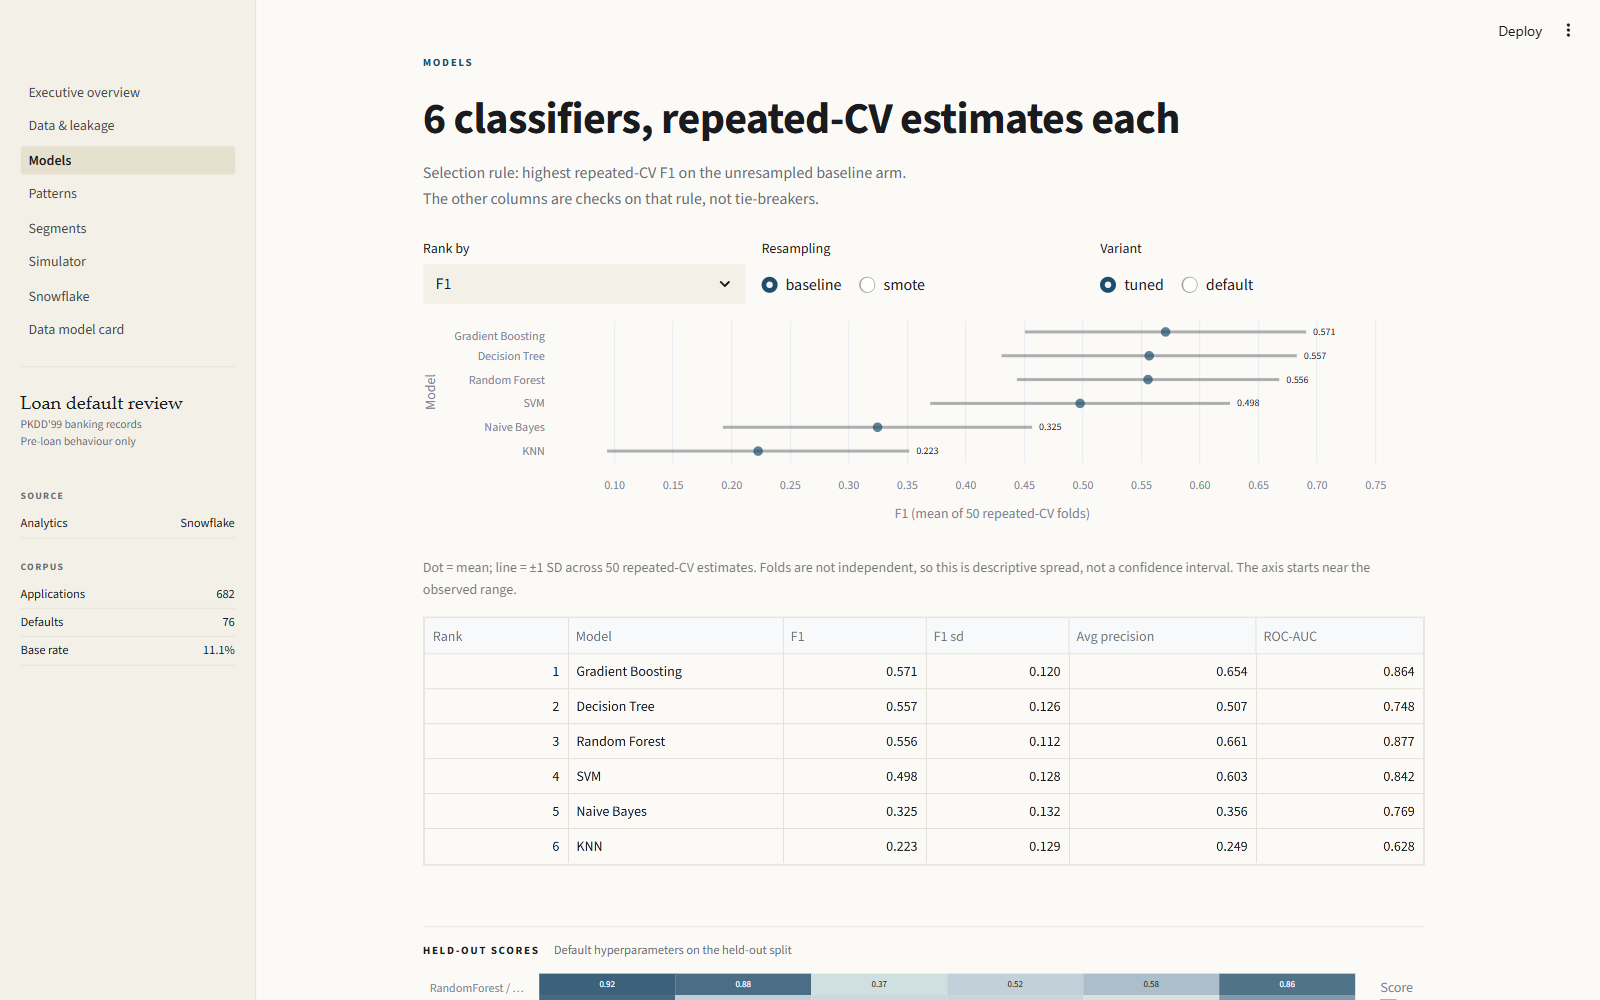
\includegraphics[width=0.92\textwidth]{figures/14_dashboard_models.png}
    \caption{Models page of the Streamlit dashboard}
    \label{fig:dashboard_models}
\end{figure}

The models page consolidates Chapter~8. A metric-aware dot plot shows the repeated-CV mean and one standard deviation for each of the 24 configurations, with a ranking table beside it. A held-out metric heatmap compares F1, average precision, and ROC-AUC across the six classifiers, and ROC and precision/recall curves are drawn for the leading models. A confusion matrix is shown at the default cutoff, tuning results quantify the gain from parameter search, and a challenger dumbbell chart compares the selected tuned Gradient Boosting model with the other algorithms. The chart makes the tied-leading result clear: the tuned Gradient Boosting model leads on F1, while Random Forest leads slightly on average precision and ROC-AUC.

\section{Patterns Page}
\begin{figure}[H]
    \centering
    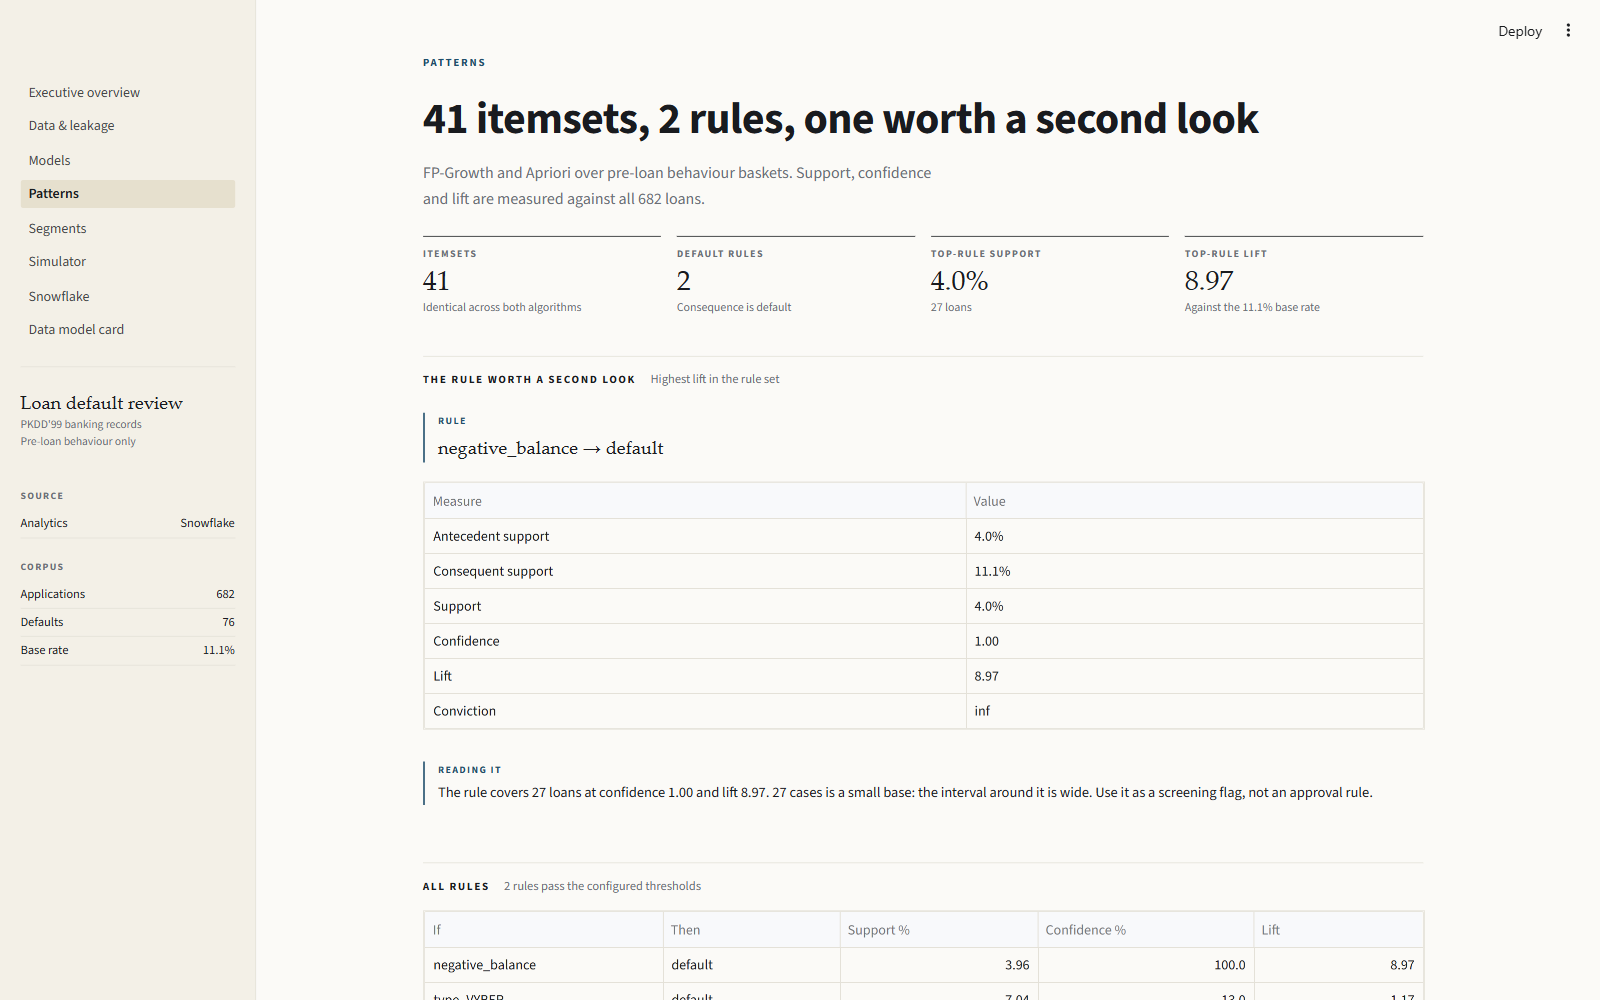
\includegraphics[width=0.92\textwidth]{figures/15_dashboard_patterns.png}
    \caption{Patterns page of the Streamlit dashboard}
    \label{fig:dashboard_patterns}
\end{figure}

The patterns page presents the association rules and the classifier-based rule list. Default rules are ranked by lift, with support and confidence shown beside them. Coverage bars for the classification-based rule set show how many defaults each rule covers, so a high-precision but low-recall rule is not mistaken for a useful screen. Itemset support bars let the jury compare Apriori and FP-Growth on the same baskets; both algorithms return 41 itemsets at a minimum support of 0.03 and a maximum length of three.

\section{Segments Page}
\begin{figure}[H]
    \centering
    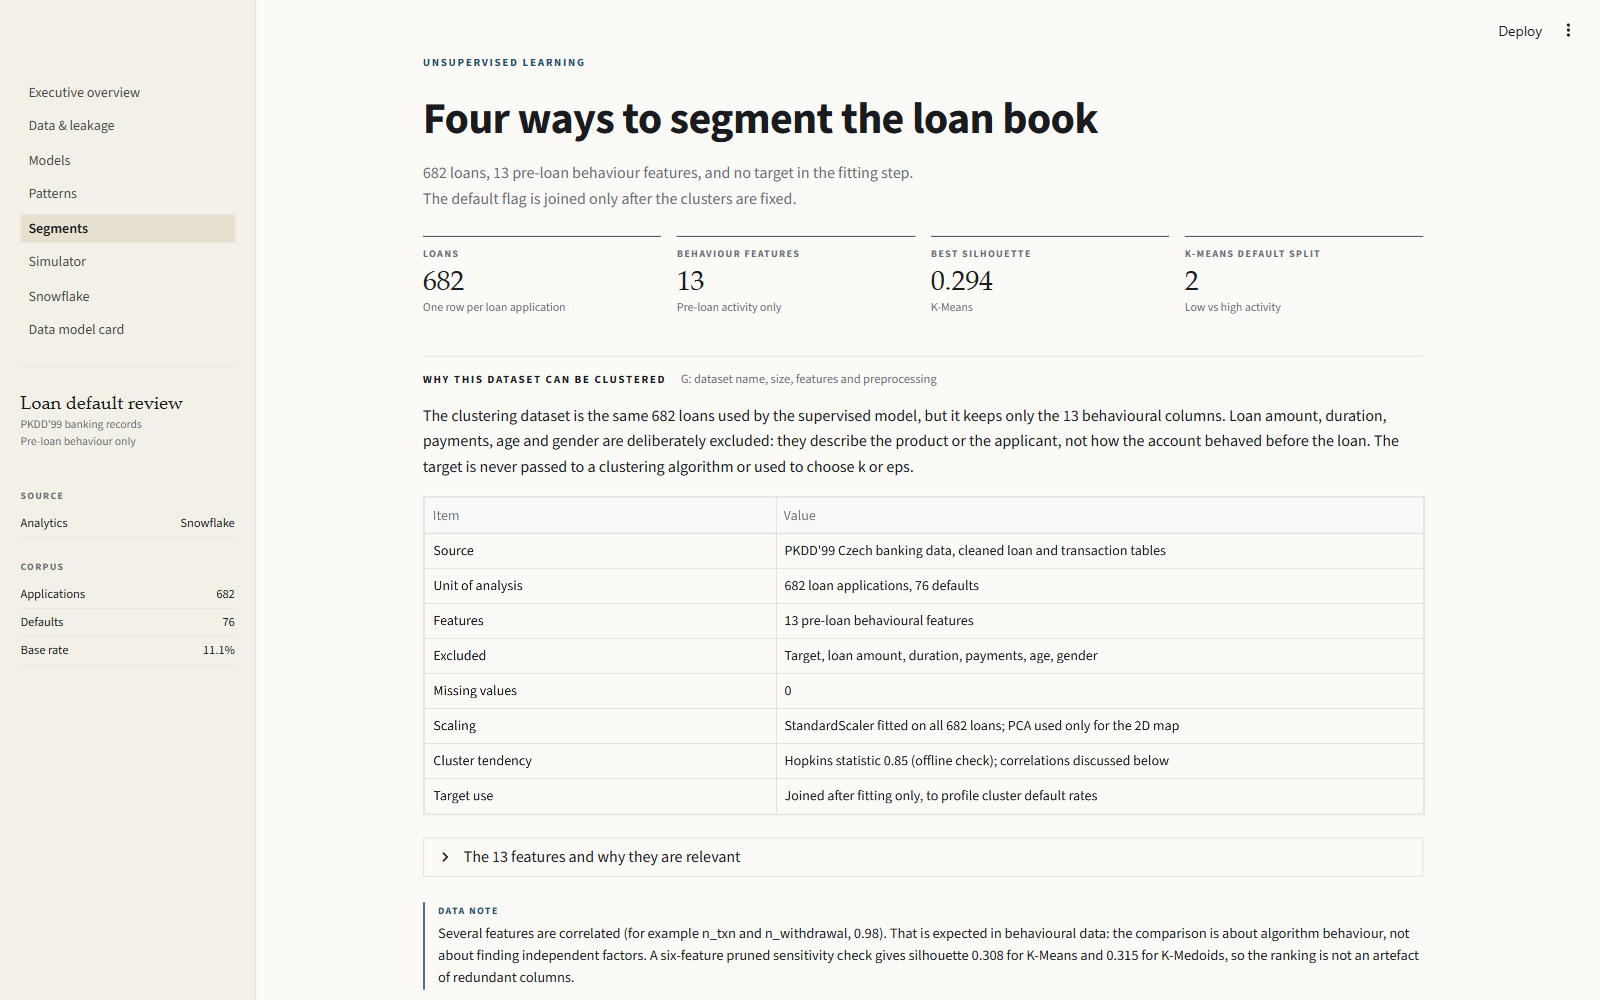
\includegraphics[width=0.92\textwidth]{figures/26_dashboard_segments.png}
    \caption{Segments page of the Streamlit dashboard}
    \label{fig:dashboard_segments}
\end{figure}

The segments page carries the unsupervised results of Chapter~9. A dataset card records that the clustering input is the 13 pre-loan behavioural features with no target. The four-algorithm comparison table is shown with its internal metrics and stability values, and charts compare those metrics visually. PCA maps display the four solutions in two dimensions, cluster profiles describe activity and balance behaviour, and a default-rate chart joins the target back for description only. The page ends with the K-Means verdict and a note that the labels are descriptive, not causal.

\section{Snowflake Deployment Page}

This page is the live counterpart of Chapter~4 and is shown in Figure~\ref{fig:snowflake_page}. It shows the RAW/MART schema split and the 20 expected objects (18 tables plus two views) with their row counts. In Snowflake mode it reads live counts and view samples and displays the verification SQL alongside them. The loader routes raw extracts into RAW and the star schema plus analytics tables into MART, truncating each target before writing so that a rerun is idempotent. This page is what a jury can open to confirm that the deployment is real rather than a diagram.

\section{Simulator Page}
\begin{figure}[H]
    \centering
    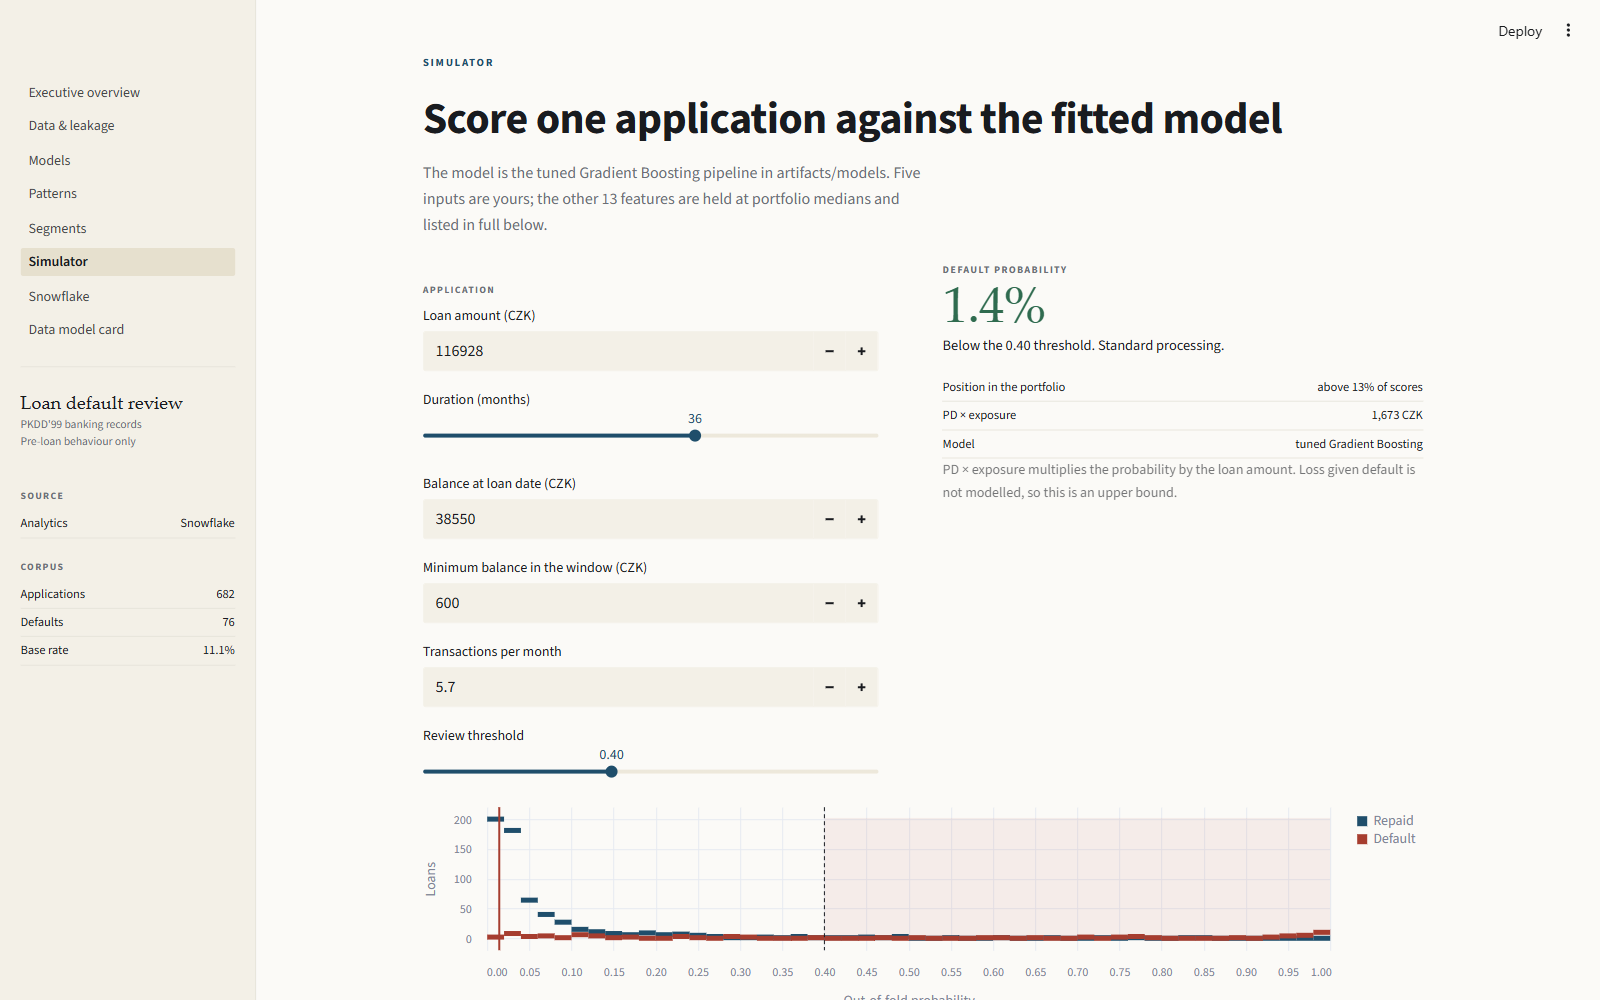
\includegraphics[width=0.92\textwidth]{figures/17_dashboard_simulator.png}
    \caption{Simulator page of the Streamlit dashboard}
    \label{fig:dashboard_simulator}
\end{figure}

The simulator scores a single application with the saved tuned Gradient Boosting pipeline. It places the resulting score against the portfolio score distribution, so an analyst can see where an applicant falls relative to the 682 historical loans. One-at-a-time stress drivers then show how the score moves when a single feature is changed while the others are held fixed. The simulator is a demonstration of the saved pipeline, not a second model, and it inherits the same restriction as the rest of the system: it supports review, not automatic rejection.

\section{Data Model Card}
\begin{figure}[H]
    \centering
    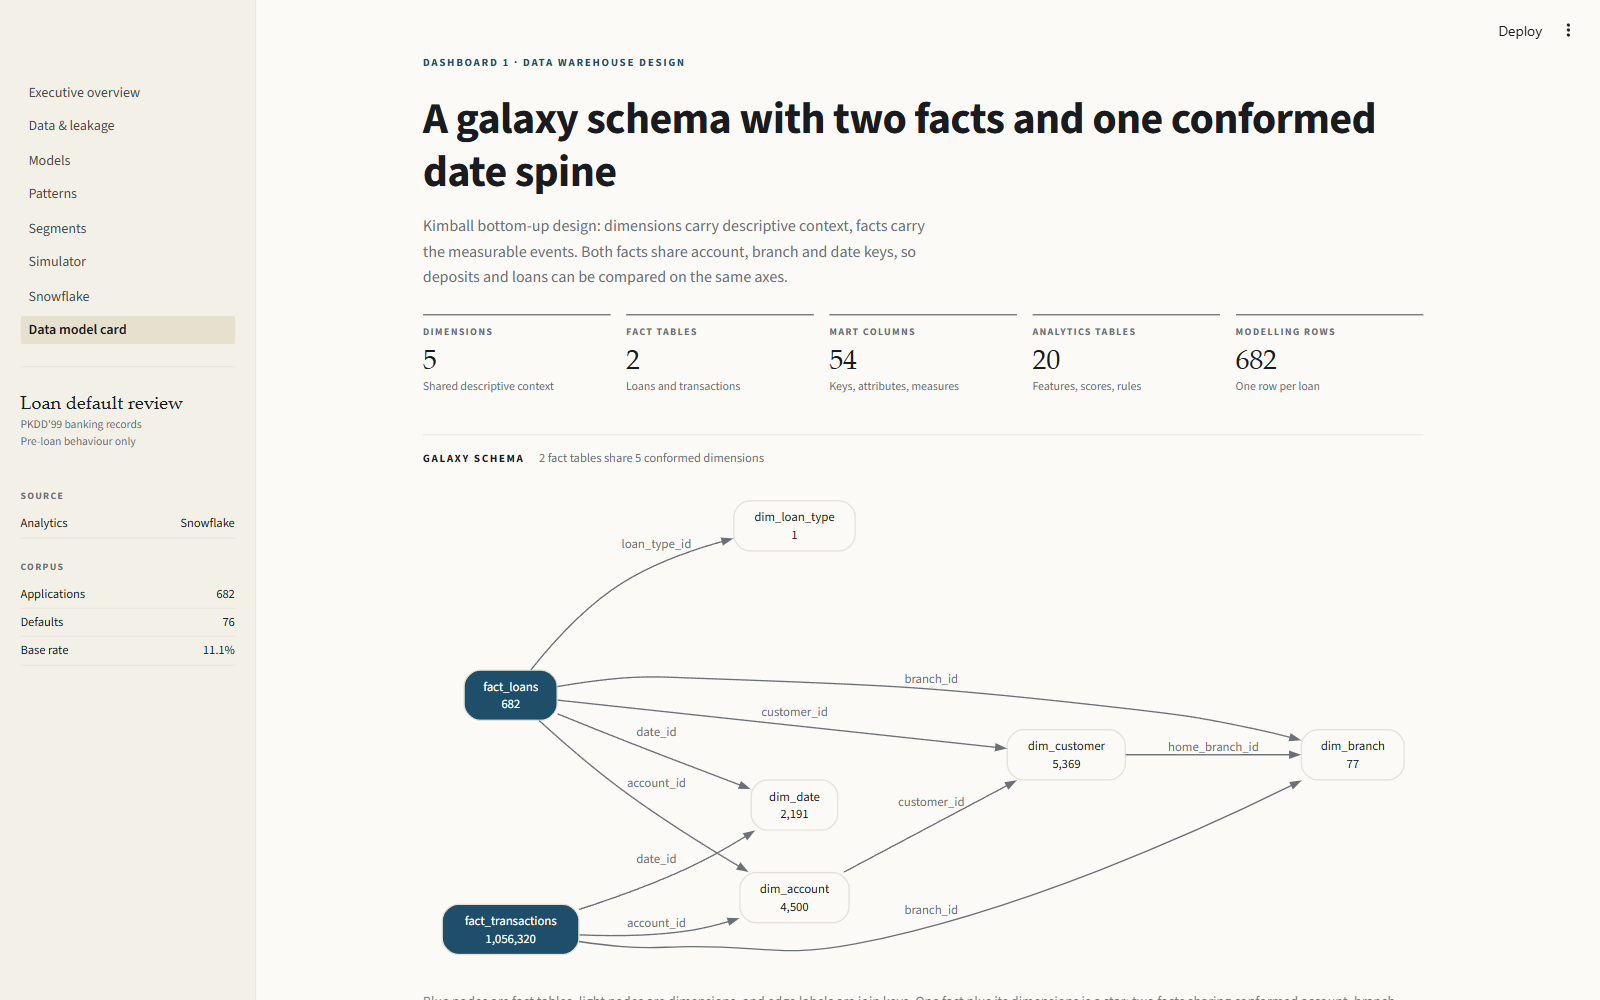
\includegraphics[width=0.92\textwidth]{figures/19_dashboard_data_model.png}
    \caption{Data model card page of the Streamlit dashboard}
    \label{fig:dashboard_datacard}
\end{figure}

The data model card is a Graphviz rendering of the galaxy schema, with an analytics row-count chart, the join keys between facts and dimensions, and a column dictionary. It is the fastest way for a jury to check that the warehouse design in Chapter~5 and the deployment in Chapter~4 describe the same objects.

\section{Jury Dashboard Map}
The jury guide asks for three dashboards mapped to rubric items. A single application supplies all three through separate pages, as shown in Table~\ref{tab:dashboard_map}.

\begin{table}[H]
    \centering
    \small
    \renewcommand{\arraystretch}{1.3}
    \begin{tabular}{|l|l|l|}
        \hline
        \textbf{Jury dashboard} & \textbf{Rubric item} & \textbf{App page} \\
        \hline
        Dashboard 1 & A $\cdot$ Data Warehouse Design & Data model card \\
        Dashboard 2 & B $\cdot$ Snowflake Deployment & Snowflake \\
        Dashboard 3 & C $\cdot$ Supervised Learning Dataset & Data and leakage \\
        \hline
    \end{tabular}
    \caption{Mapping of jury dashboards to Streamlit pages}
    \label{tab:dashboard_map}
\end{table}

The remaining rubric items are served by the other pages: classification by Models, pattern mining by Patterns, clustering by Segments, and the business recommendation by Executive overview and Simulator. Appendix~A gives the full rubric-to-evidence map.

\section{Supporting Figures}
Two static figures from the analysis are kept alongside the dashboard captures because they isolate results that the pages embed in larger layouts.

\begin{figure}[H]
    \centering
    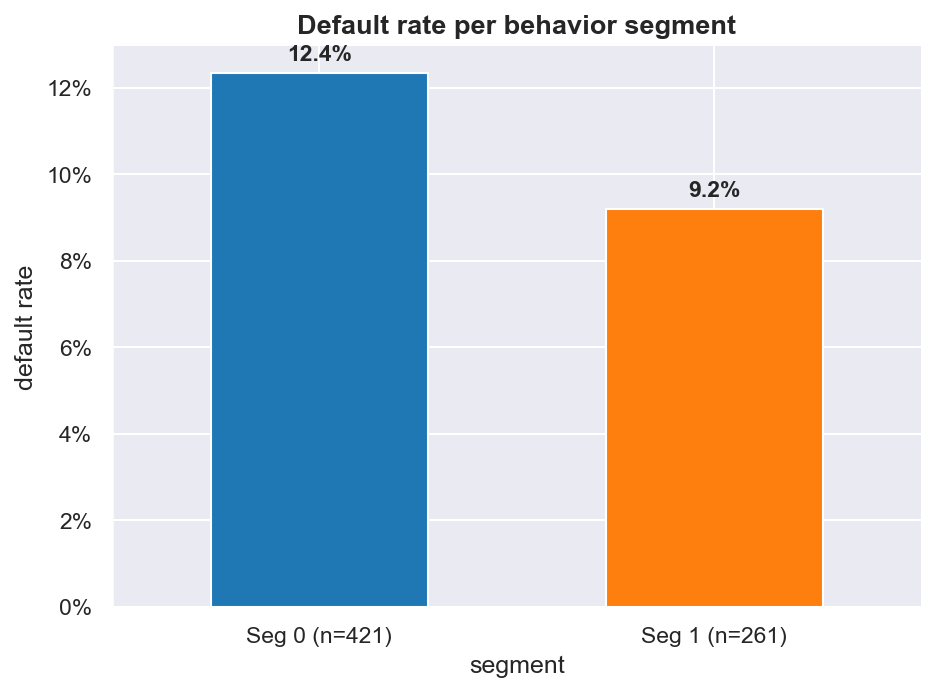
\includegraphics[width=0.88\textwidth]{figures/10_segment_default_rates.png}
    \caption{Observed default rate by behavioural segment}
    \label{fig:segment_rates_static}
\end{figure}

\begin{figure}[H]
    \centering
    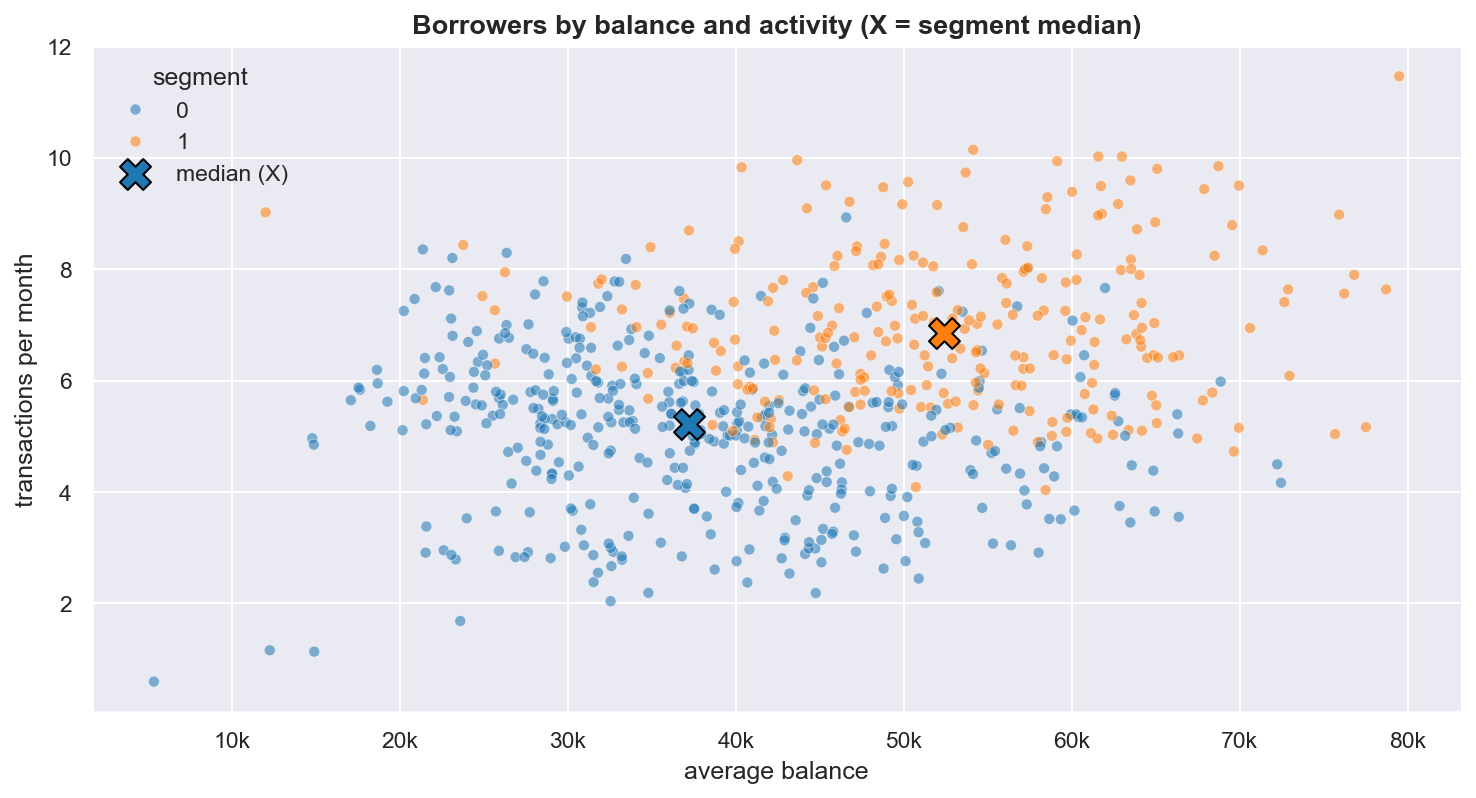
\includegraphics[width=0.88\textwidth]{figures/11_segment_scatter.png}
    \caption{Segment scatter used on the executive overview}
    \label{fig:segment_scatter_static}
\end{figure}

Together these views cover the full chain: warehouse structure, deployment evidence, leakage control, model comparison, mined rules, segments, and a single-loan score. Because every page is backed by saved artifacts rather than fresh computation, the figures in this chapter and the numbers in the earlier chapters are the same numbers.

\chapter{Conclusion and Future Scope}

\section{Summary}
This project built a complete analytics path from the raw PKDD'99 Czech banking extracts to an interactive review dashboard. The source data was reconciled to 682 loans, 1,056,320 transactions, 5,369 clients, 4,500 accounts, and 77 districts covering 1993 to 1998. A galaxy schema was modelled with two fact tables, \texttt{fact\_loans} and \texttt{fact\_transactions}, and five conformed dimensions. The warehouse was deployed to Snowflake with a RAW layer for the extracts and a MART layer for the modelled tables, together with two reporting views, \texttt{V\_LOAN\_PERF} and \texttt{V\_TRANS\_MONTHLY}. The loader truncates each target before writing, so reruns do not duplicate rows.

On top of the warehouse, a 28-column feature mart (27 columns exported for modelling) was built with a strict pre-loan rule: a transaction contributes only if \texttt{t.date\_id $<$ l.loan\_date\_id}. The check reports zero post-loan rows. Eighteen features were used for modelling: 13 behavioural aggregates, three loan terms, and two demographic attributes. Six classifiers were compared across 24 configurations under repeated five-fold cross-validation with ten repeats. The tuned Gradient Boosting model was selected with F1 $0.571 \pm 0.120$, average precision $0.654$, and ROC-AUC $0.864$, with Random Forest statistically tied on F1 and leading on the other two metrics.

Association-rule mining with Apriori and FP-Growth returned the same 41 itemsets at a support threshold of 0.03. The strongest default rule, negative balance, carries a lift of 8.97 and a precision of 1.000, but covers only 27 of the 76 defaults. Unsupervised clustering on the 13 behavioural features compared K-Means, K-Medoids, AGNES, and DBSCAN; K-Means with $k=2$ was recommended for its stability and full coverage, while DBSCAN's 129 noise loans were retained as a separate manual-review flag with a 23.26\% default rate.

All results were delivered through an eight-page Streamlit application using Altair charts and a Graphviz schema view. The application reads saved artifacts and does not retrain on load, so the displayed values match the reported ones.

\section{Contributions}
\begin{itemize}
    \item A reconciled dimensional warehouse with documented row counts, keys, and column dictionaries, deployable to Snowflake and reproducible locally.
    \item A leakage-controlled feature mart with an explicit temporal rule and a verification check that reports zero post-loan rows.
    \item A rigorous model comparison under repeated cross-validation, including class-imbalance strategies and a clear account of which strategies helped and which did not.
    \item Two independent pattern views: association rules for interpretable screens and clustering for behavioural segments, both kept separate from the supervised target until interpretation.
    \item One dashboard satisfying the three jury dashboards while also exposing the model, rule, and segmentation evidence needed by the remaining rubric items.
\end{itemize}

\section{Limitations}
The dataset contains only 76 defaults, and the held-out fold set contains about 19. Confidence intervals are therefore wide, and the tuned cross-validation estimate is slightly optimistic because the same data informed the tuning. The data ends in 1998, so the learned behaviour reflects a historical Czech banking market and may not transfer to a current portfolio. The loan type dimension has a single \texttt{Unspecified} member and the interest rate is null for every row, so product-level risk differences cannot be measured. Age and gender were available but deliberately excluded from deployment because using them as risk factors is not acceptable. The classifier-based rule set has perfect precision but low recall, so it is a review filter rather than a screening rule. The intended role of the model is a review queue: the balance screen under CZK 20{,}000 catches 34 of the 76 defaults at 35.1\% precision and flags 97 loans, which means most flagged loans are not defaulters.

\section{Future Scope}
\begin{itemize}
    \item \textbf{Refresh the data.} Newer loan vintages with labelled outcomes would narrow the confidence intervals and test whether the behavioural signals persist.
    \item \textbf{Prospective validation.} Score a forward period before deployment and compare predicted rankings with observed defaults, rather than relying only on historical cross-validation.
    \item \textbf{Richer product attributes.} Loan purpose, interest rate, and collateral would give the loan-type dimension real members and may improve discrimination.
    \item \textbf{Fairness audit.} Test error rates and review rates across protected groups before any operational use, and keep demographic attributes out of the deployed feature set.
    \item \textbf{Real-time ingestion.} The current loader is batch. A streaming layer using a managed queue and incremental warehouse tables could shorten the gap between a transaction and an updated feature.
    \item \textbf{Cloud scaling.} The same MART design could be moved to a different cloud warehouse, for example BigQuery or Redshift, if organisational standards change; this is a future option, not part of the delivered system.
    \item \textbf{Threshold policy.} Replace the fixed cutoff with a cost-based rule that weights a missed default against the analyst time spent reviewing a flagged loan.
\end{itemize}

\section{Concluding Remark}
The delivered system answers the three questions the jury guide asks. The warehouse stores the data with a documented design and a working Snowflake deployment. The supervised dataset is built without future information and produces a measurable classifier with honest uncertainty. The dashboard exposes all of it in one place. The most useful outcome is not a single accuracy figure but a defensible, inspectable pipeline whose limitations are stated as clearly as its results.


\clearpage
\phantomsection
\addcontentsline{toc}{chapter}{Appendix A: Jury Rubric Map}
\begin{center}
    {\huge \textbf{Appendix A: Jury Rubric Map}}\\[1cm]
\end{center}

\begin{table}[H]
    \centering
    \small
    \renewcommand{\arraystretch}{1.3}
    \begin{tabularx}{\textwidth}{|c|>{\raggedright\arraybackslash}X|>{\raggedright\arraybackslash}X|}
        \hline
        \textbf{Item} & \textbf{Rubric requirement} & \textbf{Report section / evidence} \\
        \hline
        A & Data Warehouse Design & Chapter 5; Fig.~\ref{fig:galaxy_schema}, Fig.~\ref{fig:dashboard_datacard}; Dashboard: Data model card \\
        \hline
        B & Snowflake Deployment & Chapter 4; Table~\ref{tab:snowflake_objects}; Dashboard: Snowflake \\
        \hline
        C & Supervised Learning Dataset & Chapter 6; Fig.~\ref{fig:feature_vector}; Dashboard: Data and leakage \\
        \hline
        D & Pattern Matching (Apriori, FP-Growth) & Chapter 7; Fig.~\ref{fig:pattern_flow}; Dashboard: Patterns \\
        \hline
        E & Classifier Comparison and Validation & Chapter 8; Table~\ref{tab:cv_results}; Dashboard: Models \\
        \hline
        F & Classification Algorithm Implementation & Chapter 8, Section 8.6; Dashboard: Simulator \\
        \hline
        G & Unsupervised Learning Dataset & Chapter 9, Section 9.2; Dashboard: Segments \\
        \hline
        H & Clustering Algorithm Comparison & Chapter 9, Section 9.4; Table~\ref{tab:clustering_compare} \\
        \hline
        I & Clustering Algorithm Implementation & Chapter 9, Sections 9.5--9.6 \\
        \hline
        J & Performance Metrics & Chapter 8, Section 8.5 and Chapter 9, Section 9.8 \\
        \hline
    \end{tabularx}
    \caption{End-semester jury rubric items A--J mapped to report sections and dashboard pages}
    \label{tab:jury_map}
\end{table}

\clearpage
\phantomsection
\addcontentsline{toc}{chapter}{References}
\begin{center}
    {\huge \textbf{References}}\\[1cm]
\end{center}

\begin{itemize}[leftmargin=1.5cm, label={}, itemsep=0.8cm]
    \item[\textbf{R1}] \textbf{Dataset}
    \begin{enumerate}[label={[\arabic*]}, leftmargin=*, labelsep=0.3cm, itemsep=0.3cm]
        \item P. Berka, ``PKDD'99 Discovery Challenge: Financial Dataset,'' 1999. [Online]. Available: \url{https://www.kaggle.com/datasets/siavashraz/1999-czech-financial-dataset}
    \end{enumerate}
    \item[\textbf{R2}] R. Kimball and M. Ross, \textit{The Data Warehouse Toolkit: The Definitive Guide to Dimensional Modeling}, 3rd ed. Hoboken, NJ, USA: Wiley, 2013.
    \item[\textbf{R3}] F. Pedregosa \textit{et al.}, ``Scikit-learn: Machine Learning in Python,'' \textit{Journal of Machine Learning Research}, vol. 12, pp. 2825--2830, 2011.
    \item[\textbf{R4}] S. Raschka, ``MLxtend: Providing machine learning and data science utilities and extensions to Python's scientific computing stack,'' \textit{Journal of Open Source Software}, vol. 3, no. 24, p. 638, 2018.
    \item[\textbf{R5}] R. Agrawal and R. Srikant, ``Fast Algorithms for Mining Association Rules in Large Databases,'' in \textit{Proc. 20th Int. Conf. Very Large Data Bases (VLDB)}, 1994, pp. 487--499.
    \item[\textbf{R6}] J. Han, J. Pei, and Y. Yin, ``Mining Frequent Patterns without Candidate Generation,'' in \textit{Proc. ACM SIGMOD Int. Conf. Management of Data}, 2000, pp. 1--12.
    \item[\textbf{R7}] L. Breiman, ``Random Forests,'' \textit{Machine Learning}, vol. 45, no. 1, pp. 5--32, 2001.
    \item[\textbf{R8}] Snowflake Inc., ``Snowflake Documentation -- Databases, Schemas and Views.'' [Online]. Available: \url{https://docs.snowflake.com/}
    \item[\textbf{R9}] Streamlit Inc., ``Streamlit Documentation -- Data Apps in Python.'' [Online]. Available: \url{https://docs.streamlit.io/}
\end{itemize}

\end{document}
